
\RequirePackage{amsmath}
\documentclass[useAMS, usenatbib]{mnras}

% The following is needed to fix the margins if using Letter-size paper
% REMOVE if your LaTeX uses A4 paper by default
%\addtolength\topmargin{-1.8cm}

% Standard LaTeX packages
% \usepackage[varg]{txfonts}
\usepackage[varg]{newtxmath}
\usepackage{newtxtext}
\usepackage{graphicx}
\usepackage{microtype}
\usepackage{xcolor}
\usepackage{fixltx2e}
\usepackage{booktabs}
\usepackage{hyperref}
\usepackage{siunitx}
\usepackage{color}
\usepackage{appendix}
\hypersetup{colorlinks=True, linkcolor=blue!50!black, citecolor=black,
  urlcolor=blue!50!black}

%% Bold italic
\newcommand\hmmax{0}            % we don't need heavy fonts
\newcommand\bmmax{1}            % reduce use of math alphabets for bold
\usepackage{bm}

%% Bundled custom packages
\usepackage{aastex-compat}
%\usepackage{astrojournals}


\title[Bowshock shapes]{True versus apparent shapes of astrophysical bow shocks}

\newcommand\AddressCRyA{Instituto de Radioastronom\'{\i}a y Astrof\'{\i}sica,
  Universidad Nacional Aut\'onoma de M\'exico, Apartado Postal 3-72,
  58090 Morelia, Michoac\'an, M\'exico}
\author[Tarango Yong \& Henney]{
  Jorge A. Tarango Yong \& William J. Henney\\
  \AddressCRyA
}
\begin{document}
\maketitle
\begin{abstract}
  We develop a general framework for the effects of viewing angle on
  the apparent shape of a limb-brightened, cylindrically symmetric
  curved shock (bow shock).  
\end{abstract}

\section{Introduction}
\label{sec:intro}

%%
%% Circumstances when bowshocks arise
%%

The archetypal bow shock is formed when a solid body moves
supersonically through a compressible fluid.  Terrestrial examples
include the atmospheric re-entry of a space capsule, or the sonic boom
produced by a supersonic jet \citep{van-Dyke:1982a}.  In astrophysics
the term bow shock is employed more widely, to refer to many different
types of curved shocks that have approximate cylindrical symmetry.
Instead of a solid body, astrophysical examples usually involve the
interaction of \emph{two} supersonic flows, such as the situation of a
stellar wind emitted by a star that moves supersonically through the
interstellar medium \citep{van-Buren:1988a, Kobulnicky:2010a,
  van-Marle:2011a, Mackey:2012b, Mackey:2015a}.  In such cases, two
shocks are generally produced, one in each flow.  Sometimes,
especially in heliospheric studies \citep{Zank:1999a, Scherer:2014a}, the
term ``bow shock'' is reserved for the shock in the ambient medium,
with the other being called the ``wind shock'' or ``termination
shock''.  However, in other contexts such as colliding wind binaries
\citep{Stevens:1992a, Gayley:2009a} such a distinction is not so
useful.  In this paper we use the term ``bow shock'' in a more general
sense to refer to either of the two shocks, or to the shocked gas in
between them. 


%% 
%% Examples of astrophysical bowshocks
%%

%% 
%% Restriction to cylindrical symmetry
%% 

For simplicity, the current paper is restricted to cylindrically
symmetric bowshock shapes. 

%%
%% Effects of instabilities
%%


%%% Local Variables:
%%% mode: latex
%%% TeX-master: "proplyd-bowshocks"
%%% End:

\section{Generic bow shock model}
\label{sec:generic-model}

\begin{figure}
% 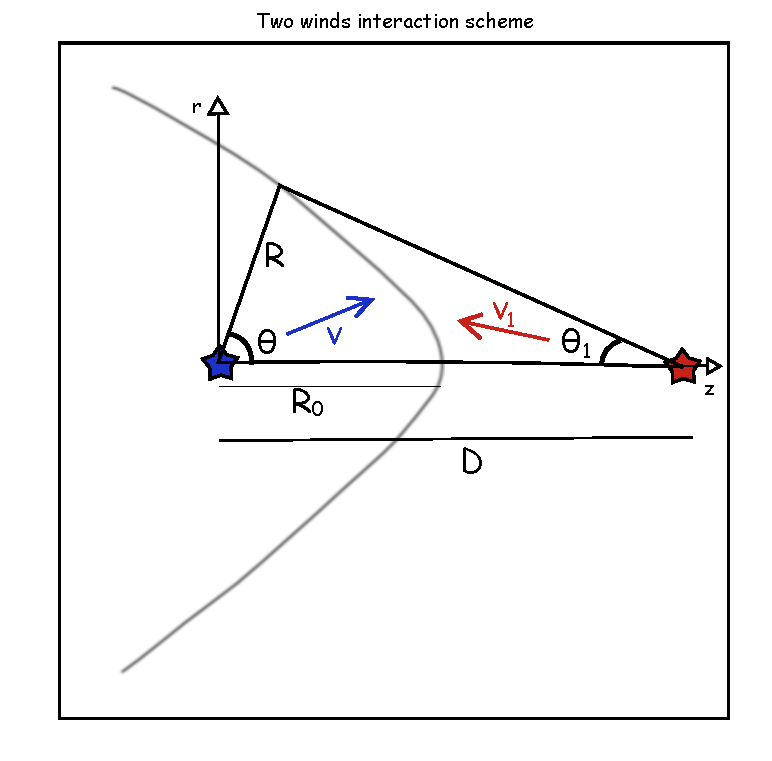
\includegraphics[width=\linewidth]{2winds-scheme}
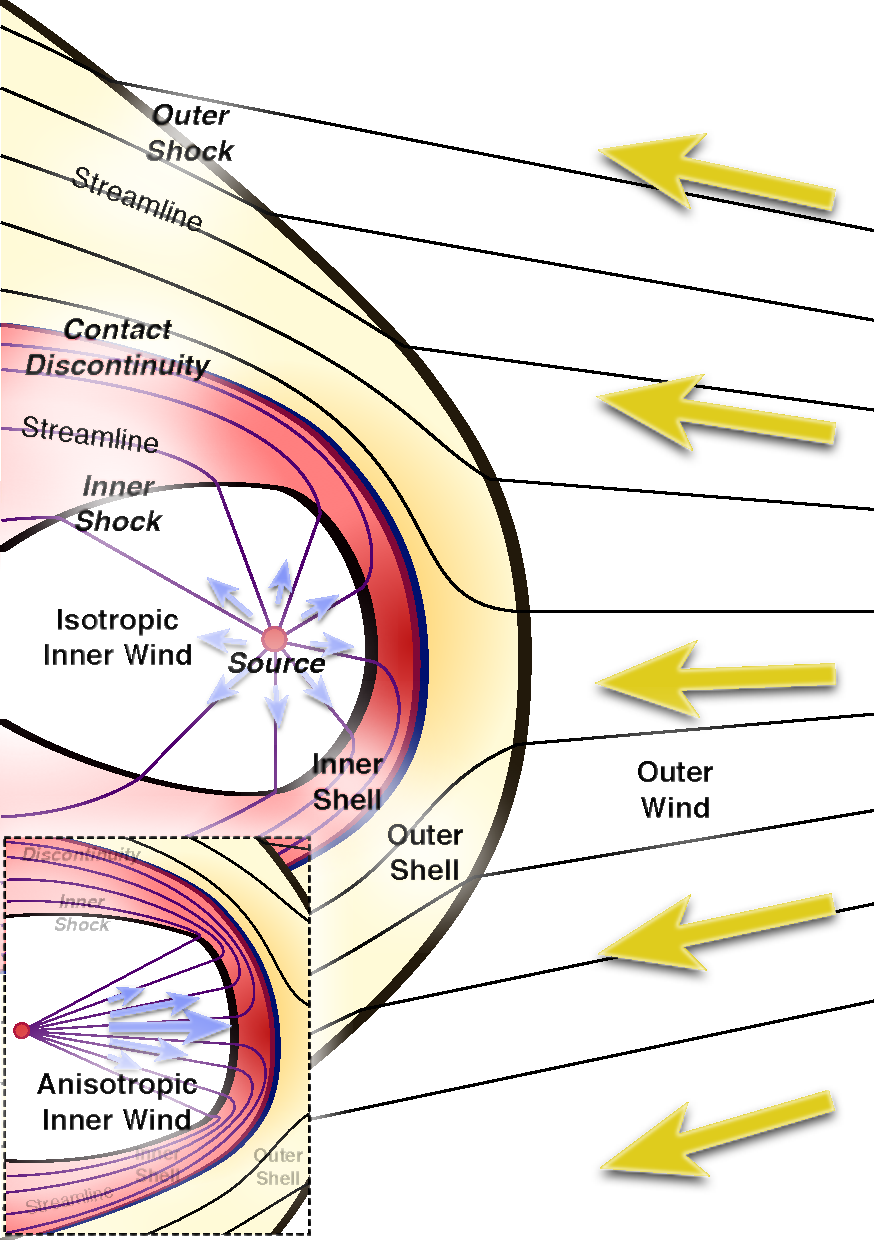
\includegraphics[width=\linewidth]{figs/generic-bowshock}
\caption{Quasi-stationary bow shock structure formed by the
  interaction of two supersonic winds.  Lower-left inset box shows the
  case where the inner wind is anisotropic.   
  % the two winds problem. Any point in the shell is located with the
  % coordinates $(R,\theta)$, and $\theta_1$ is measured from the
  % external wind position
}
\label{fig:2-winds}
\end{figure}

The general case of a two-wind interaction bow shock is illustrated in
Figure~\ref{fig:2-winds}.  If the winds are isotropic, then the bow
shock pattern wraps around the weaker of the two sources, in 

The bow shocks we consider are originated by a source located at the origin, emitting a wind with a mass loss rate of $\dot{M}_w$ and a terminal
(supersonic) velocity $v_w$. This wind interacts with another wind originated by another source located at a distance $D$ from the first one. 
The mass loss rate of the second source is $\dot{M}_{w1}$ and the terminal velocity is $v_{w1}$. The momentum of the wind of the second source is
higher than the momentum of the first one, and the resultant bow shock is stationary due to pressure balance. 

\subsection{Characteristic Radii}

In order to contrast different bow shock models, we  derive a set of measurable radii. Each model used should predict them and these predictions can be
compared with observations.

\begin{itemize}
\item Radius at axis of symmetry. Denoted as $R_0$. 
\item Radius of Curvature at the axis of symmetry. Denoted as $R_c$
\item Radius at the  perpendicular direction to the symmetry axis. Denoted as $R_{90}$
\item For open bow shocks, the asymptotic angle. Denoted as $\theta_\infty$
\end{itemize} 

\begin{figure}
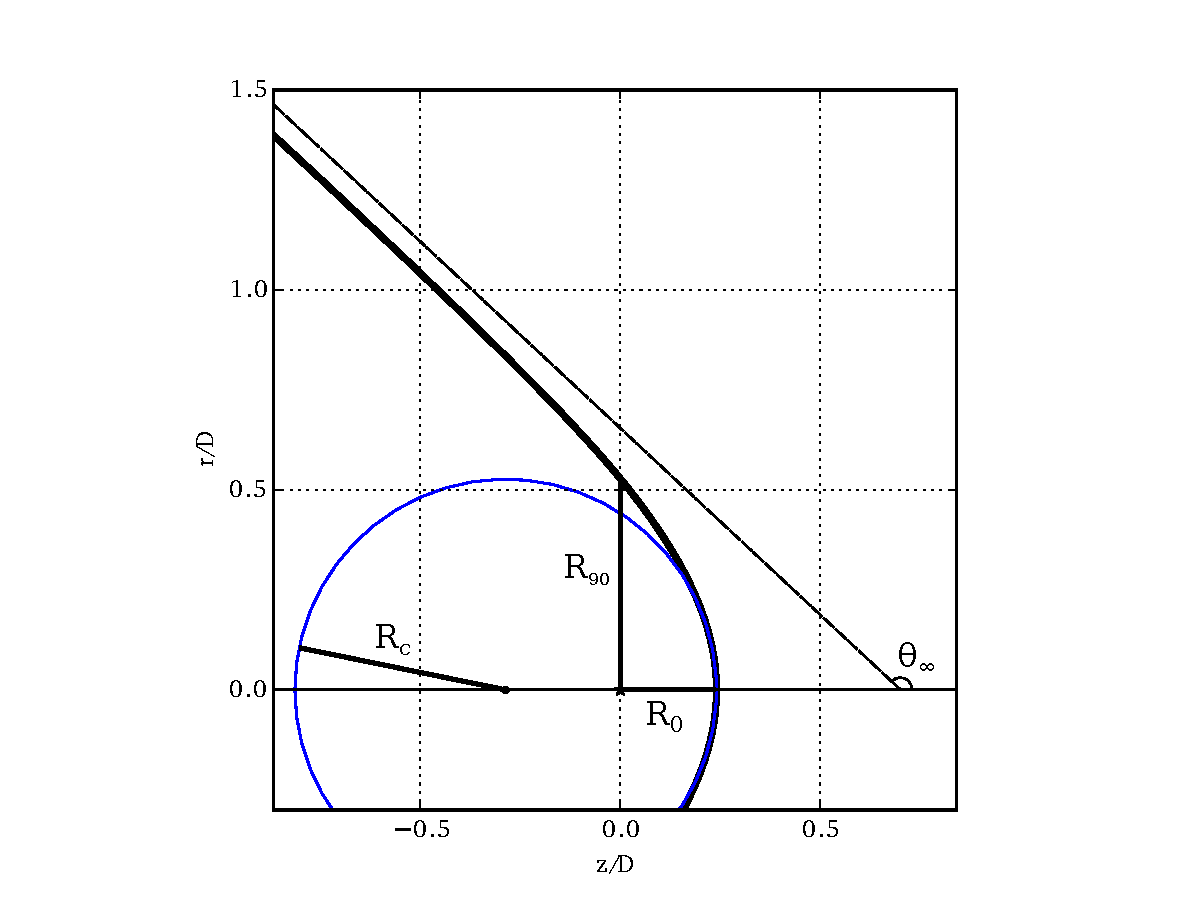
\includegraphics[width=\linewidth]{ch-radii_ed2}
\caption{Schematic representation of the characteristic radii $R_0$, $R_{90}$ and the radius of curvature at the symmetry axis $R_c$}
\end{figure}



%%% Local Variables:
%%% mode: latex
%%% TeX-master: "proplyd-bowshocks"
%%% End:

\newenvironment{Vector}{\left(\begin{array}{c}}{\end{array}\right)}
\newcommand\uvec[1]{\bm{\hat{#1}}}
\newcommand\T{_{\mathrm{\scriptscriptstyle T}}}

\section{Projection onto the plane of the sky}
\label{sec:projection}

In this section we calculate the apparent shape on the plane of the
sky of the limb brightened border of a shock or shell that is
idealized as an arbitrary cylindrically symmetric surface.

%Note: I'm aware that some of this material should be moved to an appendix, but I think it will be a future edition.
\subsection{Frames of reference}
\label{sec:ref-frames}

Consider body-frame cartesian coordinates $(x,y,z)$, where \(x\) is
the symmetry axis, and spherical polar coordinates
\((R, \theta, \phi)\), where \(\theta\) is the polar angle and
\(\phi\) the azimuthal angle.  Since the surface is cylindrically
symmetric, it is can be specified as $R = R(\theta)$, so that
cartesian coordinates on the surface are:
\begin{equation}
  \begin{Vector}
    x \\ y \\ z
  \end{Vector} 
  = R(\theta)
  \begin{Vector}
    \cos\theta \\
    \sin\theta\cos\phi \\
    \sin\theta\sin\phi
  \end{Vector}.
  \label{eq:body-frame}
\end{equation} 
Suppose that the viewing direction makes an angle \(i\) with the
\(z\)~axis, so that we can define observer-frame coordinates
\((x', y', z')\), which are found by rotating the body-frame
coordinates about the \(y\)~axis:
\begin{equation}
  \begin{Vector}
    x' \\ y' \\ z'
  \end{Vector}
  = 
  \begin{Vector}
    x\cos i - z\sin i\\
    y \\
    z\cos i + x\sin i
  \end{Vector}.
  \label{eq:Trans}
\end{equation} 
The relationship between the two frames is illustrated in
Figure~\ref{fig:projection-pos}.  All quantities in the observer's
frame are denoted by attaching a prime to the equivalent quantity in
the body frame.  The celestial coordinates on the ``plane of the sky''
are given by \((x', y')\) with \(x'\) being the projected symmetry
axis of the surface, while the line of sight lies along \(-z'\).  The
inclination angle \(i\) is defined so that \(i = 0^\circ\) when the
surface is viewed perpendicular to its axis (\textit{side on}) and
\(i = 90^\circ\) when it is viewed along its axis (\textit{end on}).

\begin{figure}
  \centering
  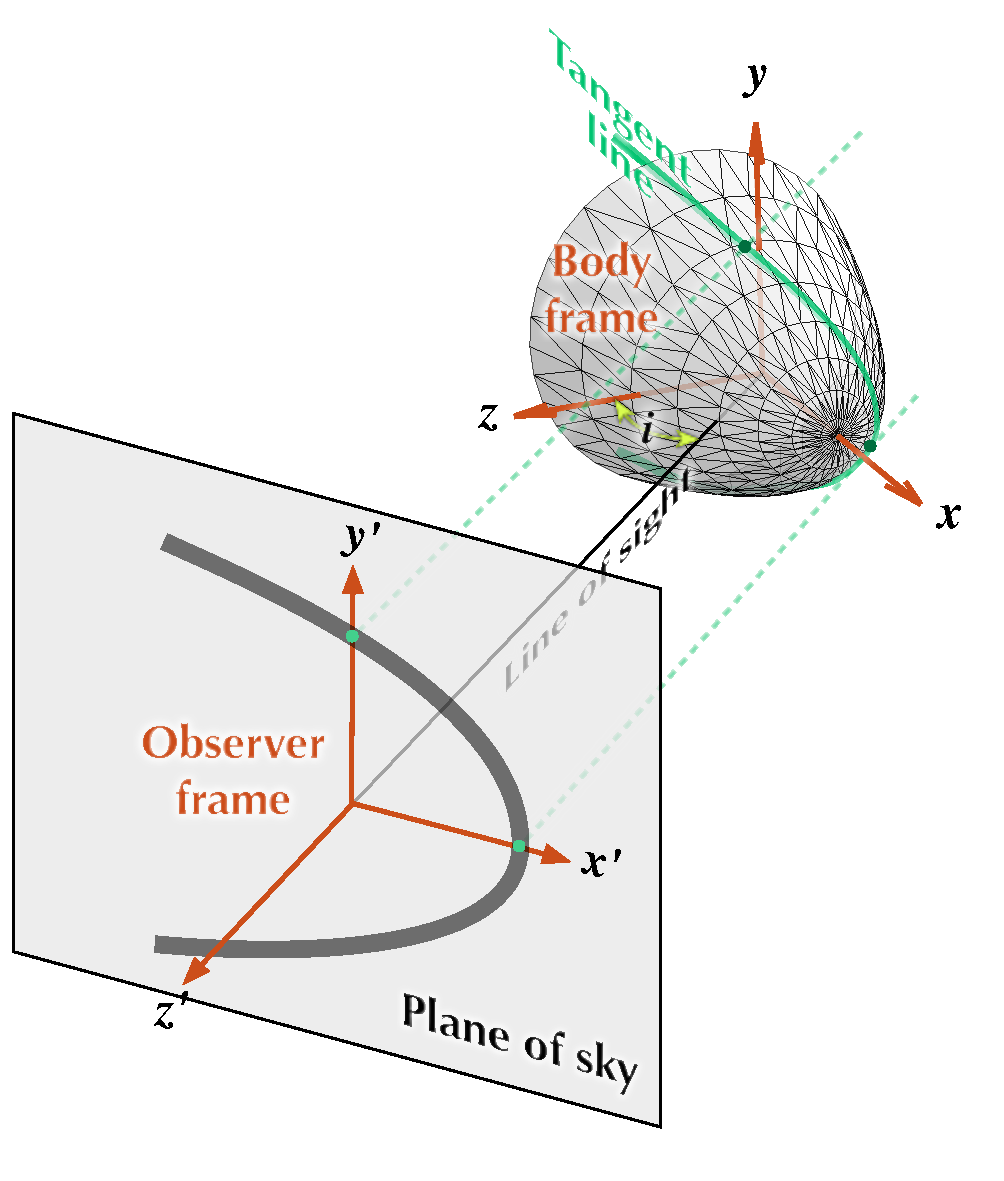
\includegraphics[width=\linewidth]{figs/projection-pos}
  \caption{Relationship between body frame (unprimed coordinates) and
    observer frame (primed coordinates).}
  \label{fig:projection-pos}
\end{figure}


%\subsection{Characteristic radii}
%\label{sec:characteristic-radii}
\begin{figure}
  \centering
  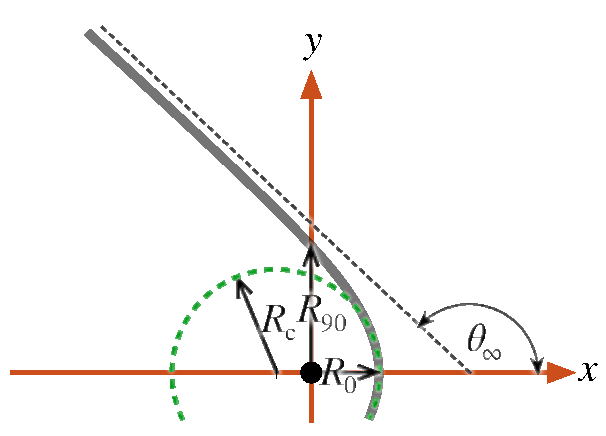
\includegraphics[width=\linewidth]{figs/characteristic-radii}
  \caption{Characteristic radii in the body frame.}
  \label{fig:characteristic-radii}
\end{figure}

\subsection{Unit vectors normal and tangential to the surface}
\label{sec:unit-vectors-normal}
\begin{figure}
  \centering
  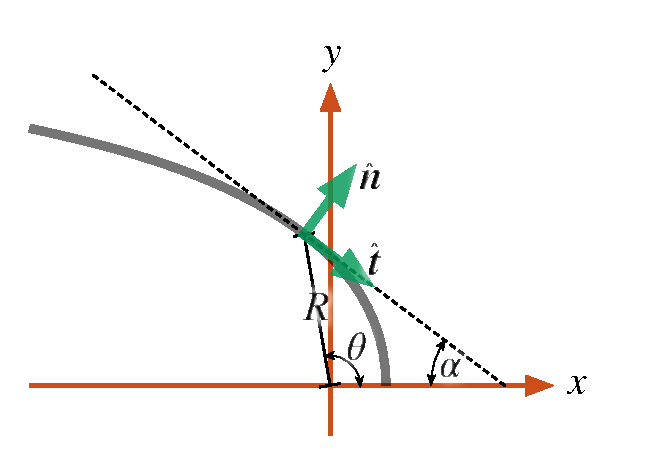
\includegraphics[width=\linewidth]{figs/bowshock-unit-vectors}
  \caption{Unit vectors in the body frame that are normal and
    tangential to the surface \(R(\theta)\) in a plane of constant
    azimuth, \(\phi\).}
  \label{fig:unitvec}
\end{figure}
We define unit vectors \(\uvec{n}, \uvec{t}\), such that \(\uvec{n}\) is normal to the surface, while \(\uvec{t}\) is tangent to the surface in a plane of constant \(\phi\). For \(\phi = 0\) the surface lies in the \(xy\) plane and it is straightforward to show (Fig.~\ref{fig:unitvec}) that in this case the unit vectors are given by 
\begin{equation}
  \label{eq:uvec-phi0}
  \uvec{t}_0 =
  \begin{Vector}
    -\cos\alpha \\ \sin\alpha \\ 0
  \end{Vector}
  \quad \mathrm{and} \quad
  \uvec{n}_0 =
  \begin{Vector}
    \sin\alpha \\ \cos\alpha \\ 0
  \end{Vector}, 
\end{equation}
where
\begin{equation}
  \label{eq:alpha}
  \tan\alpha = -\left.\frac{dy}{dx}\right\vert_{R(\theta)} 
  = \frac{1 + \omega \tan\theta}{\tan\theta - \omega}
\end{equation}
and 
\begin{equation}
  \label{eq:omega}
  \omega(\theta) = \frac{1}{R} \frac{dR}{d\theta} . 
\end{equation}
For general \(\phi\), \(\uvec{n}\) and \(\uvec{t}\) can be found by rotating equations~(\ref{eq:uvec-phi0}) around the \(x\)-axis, which can then be converted to the observer frame by use of equation~(\ref{eq:Trans}) to give
\begin{gather}
  \label{eq:nprime}
  \begin{split}
    \uvec{n}' = & \frac{1}{(1+\omega^2)^{1/2}} \\
    & \times 
      \begin{Vector}
        (\cos\theta+\omega\sin\theta)\cos i 
        - (\sin\theta-\omega\cos\theta) \sin i \sin\phi\\
        (\sin\theta-\omega\cos\theta)\cos\phi \\
        (\cos\theta+\omega\sin\theta)\sin i 
        + (\sin\theta-\omega\cos\theta)\sin\phi\cos i
      \end{Vector}\\
  \end{split}\\
  \label{eq:tprime}
  \begin{split}
    \uvec{t}' = & \frac{1}{(1+\omega^2)^{1/2}} \\
    & \times 
      \begin{Vector}
        -(\sin\theta-\omega\cos\theta)\cos i
        - (\cos\theta+\omega\sin\theta)\sin\phi\sin i \\
        (\cos\theta+\omega\sin\theta)\cos\phi \\
        -(\cos\theta+\omega\sin\theta)\sin i 
        + (\sin\theta-\omega\cos\theta)\sin\phi\cos i
      \end{Vector}
  \end{split}
  \end{gather}
\subsection{Tangent line}

% For optically thin emission with isotropic emissivity \(j\), the observed
% surface brightness for any line of sight that intersects the shell is
% \(S = \int j \, dz' / 4\pi\). 
 
% If the shell thickness is \(h(\theta)\) and emissivity is
% \(j(\theta)\), then for optically thin emission the observed
% surface brightness for any line of sight that intersects the shell is
% \(S = j s / 4\pi\), where \(s\)

% in the limit \(h \ll R\) and
% \(\mu\) is
% the cosine of the angle between the line of sight and the local normal
% to the shell surface at the point of intersection:
% \begin{equation}
%   \label{eq:2}
%   \mu = \uvec{n} \cdot \uvec{z}'
% \end{equation}

The boundary on the plane of the sky of the projected surface is the
locus of those lines of sight that graze the surface tangentially.
This corresponds to a curved line on the surface itself, which we
denote the \textit{tangent line}, and which is defined by the
condition  
\begin{equation}
  \label{eq:tangent-line-condition}
  \uvec{n}'\cdot \uvec{z}' = 0.
\end{equation}


We denote by \(\phi\T\) that value of $\phi$ that satisfies this
relation for a given inclination, \(i\), and polar angle, \(\theta\):
\begin{equation}
\sin\phi\T = \tan i\tan\alpha = \tan i \frac{1+\omega\tan\theta}{\omega-\tan\theta}
\label{eq:tanphi}
\end{equation}
From equations~(\ref{eq:body-frame}, \ref{eq:Trans}) it follows that
the observer-frame coordinates of the tangent line are given by
\begin{equation}
\left(\begin{array}{c}
x'\T \\ y'\T \\ z'\T
\end{array}\right)= R(\theta)\left(\begin{array}{c}
\cos\theta\cos i - \sin\theta\sin\phi\T \sin i \\
\sin\theta(1-\sin^2\phi\T)^{1/2} \\
\cos\theta\sin i +\sin\theta\sin\phi\T\cos i
\end{array}\right).
\label{eq:tangential}
\end{equation} 
Note that, in general, \(z'\T\) is not a linear function of \(x'\T\)
and \(y'\T\), so that the tangent line is not a plane curve. 

The apparent shape \((x'\T, y'\T)\) of the tangent line on the plane
of the sky can also be described in polar form as \(R'(\theta')\),
where
\begin{equation}
  \label{eq:R-prime-theta-prime}
  R' = (x'^2\T+ y'^2\T)^{1/2} 
  \quad \text{and} \quad
  \tan\theta' = y'\T / x'\T.
\end{equation}
It is important to note that equation~(\ref{eq:tanphi}) does not have
a solution for arbitrary values of $\theta$ and $i$, but only when
$|\tan i\tan\alpha|<1$. In particular, if $i\neq 0$, then the tangent
line only exists for \(\theta > \theta_{0}\) where \(\theta_{0}\) is
given implicitly by
\begin{align}
\tan\theta_{0} = \frac{|\tan i| + \omega(\theta_{0})}{1-\omega(\theta_{0}) |\tan i|} . 
\label{eq:thetapar}
\end{align}
In addition, if the surface is sufficiently ``open''
(\(\alpha > \alpha_{\mathrm{min}} > 0\) for all \(\theta\)), then for
those inclinations with
\(\vert i\vert > (90^\circ - \alpha_{\mathrm{min}}) \) the tangent
line does not exist for any value of \(\theta\).  In other words, when
the viewing angle is sufficiently close to face-on, the projected
surface has no ``edge'' and will no longer appear to be a bow shock.

\subsection{Characteristic radii on the plane of the sky}

Considering further applications to bow shocks, we will consider open shells. In order to compare the shell shape given by $R(\theta)$ with observations,
it is convenient to define the following apparent radii in the observer frame: $R'_{0}$ and $R'_{90}$. These are projected distances of the shell tangent line
from the origin. The first is measured in the direction of the symetry axis, and the second in a perpendicular direction. More concretely $R'_{0} = x'\T(y'\T=0)$
and $R'_{90} = y'\T(x'\T=0)$. From equations (\ref{eq:tanphi}) and (\ref{eq:tangential}) we find that:
\begin{align}
R'_{0} = R(\theta_{0})\cos(\theta + i) \label{eq:Rpar} 
\end{align}
Where $\theta_{0}$ is the solution of equation (\ref{eq:thetapar}), and
\begin{align}
R'_{90} = R(\theta_{90})\sin\theta_{90}\left(1-\sin^2(\phi\T(\theta_{90}))\right)^{1/2}
\end{align}
Where $\theta_{90}$ is the solution of the next implicit equation:
\begin{align}
\cot\theta_{90} = \frac{1-\left(1+\omega(\theta_{90})^2\sin^22i\right)^{1/2}}{2\omega(\theta_{90})\cos^2 i}
\end{align}


  \subsection{Line-of-sight velocities on the tangent line}
  \label{sec:line-sight-veloc}
  Motions in a thin shocked shell will be predominantly tangential to the shell surface. In addition, for the particular case of wind-wind bowshocks, the flow in each azimuthal slice can be shown to be independent \citep{Wilkin:2000a}, which implies that the shell velocity is parallel to \(\uvec{t}\). The projected line-of-sight shell velocity is therefore
  \begin{equation}
    \label{eq:vlos}
    v_{\mathrm{los}} = (\uvec{t}' \cdot -\uvec{z}') \, v_{\parallel}(\theta) = \frac{v_{\parallel}(\theta) (1+\omega^2)^{1/2} \sin i }{\sin\theta - \omega\cos\theta} ,
  \end{equation}
  where \( v_{\parallel}(\theta)\) is the gas velocity along the shell and the standard sign convention has been adopted such that velocities away from the observer are deemed positive. 


%%% Local Variables:
%%% mode: latex
%%% TeX-master: "proplyd-bowshocks"
%%% End:


\section{Conic section approximation to bow shock shapes}
\label{sec:conic}

\newcommand\Sin{\ensuremath{\mathcal{S}}}
\newcommand\Cos{\ensuremath{\mathcal{C}}}
\newcommand\Cot{\ensuremath{\mathcal{T}}}

In this section we will analyze the case where the resultant shape  of the bow shock is a conic curve (circle, ellipse, parabola or hyperbola).
These curves are mathematical simple to model and give us a good reference to understand the effects of the projection effects
described in the last section on other bow shocks. The source of the inner wind is located at the origin, and the center of the conic is located at
a distance $x_0$ from the source.

%Instead of the excentricity, we utilize the parameter $\theta_c$ to characterize the different curves, where
%$\tan\theta_c = \frac{b}{a}$,  $b$ and $a$ are the typical parameters of conics. A positive value for $\theta_c$ indicates that the given curve is a closed one, i.e
%an ellipse, while a negative value indicates that is an hyperbola. %Insert figures if neccesary  
\begin{figure}
\begin{tabular}{cc}
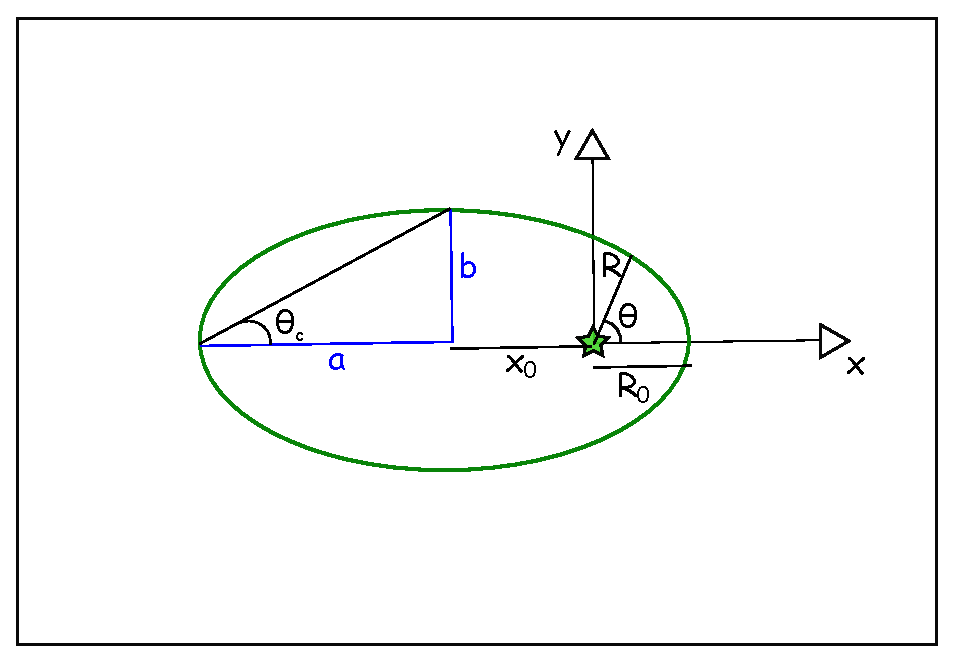
\includegraphics[width=0.4\linewidth]{ellipse} &
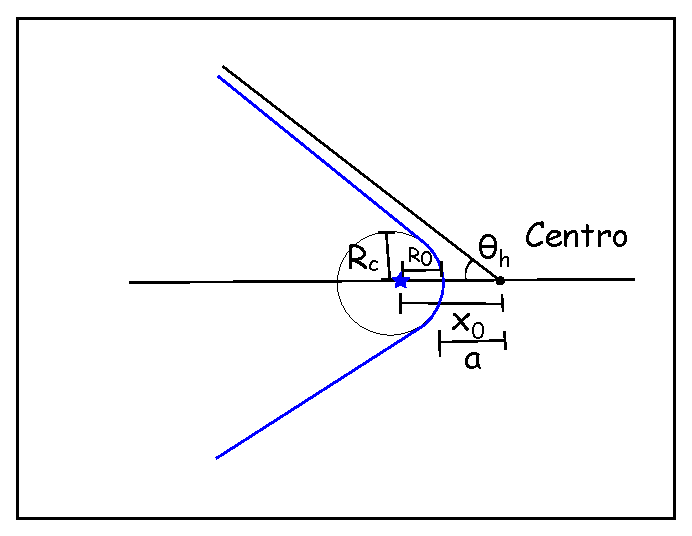
\includegraphics[width=0.4\linewidth]{hiperbola}
\end{tabular}
\label{fig:conics}
\caption{Schematic representation of conic like bowshocks: A) Ellipse and B) Hyperbola The center of the conic is located at a distance $x_0$ from the origin at the $x$ axis. The shell position is 
described either by cartesian coordinates $(x,y)$ or polar coordinates $(R,\theta)$. In this section is more convenient to use cartesian coordinates, as their parametrization is quite easy.}
\end{figure}
Due to the similitudes between the parametrization of the ellipse and the hyperbola, we can do the following parametrization:

\begin{align}
x = a\Cos(t)-x_0 \\ 
y = b\Sin(t)
\end{align}

where:
\begin{align}
\Cos(t) = \left\lbrace \begin{array}{c}
\cos t ~\mathrm{if~ellipse} \\
\cosh t ~\mathrm{if~hyperbola}
\end{array}\right.\\
\Sin(t) = \left\lbrace \begin{array}{c}
\sin t ~\mathrm{if~ellipse} \\
\sinh t ~\mathrm{if~hyperbola}
\end{array}\right. \\
-\pi < t < \pi \\
R_0 = a - x_0 \\
a<0 ~ \mathrm{for~hyperbola}
\end{align}
We have set a whole family of curves with a singular parameter denoted as $\tan\theta_c \equiv \frac{b}{a}$. Positive values of this parameter describe closed curves
(i.e. ellipses) and the negative ones describe open curves (i.e. hyperbolas). Particular cases are $\theta_c =\frac{\pi}{4}$, which describes a circle and $\theta_c=0$, which describes
a parabola.
\begin{figure}
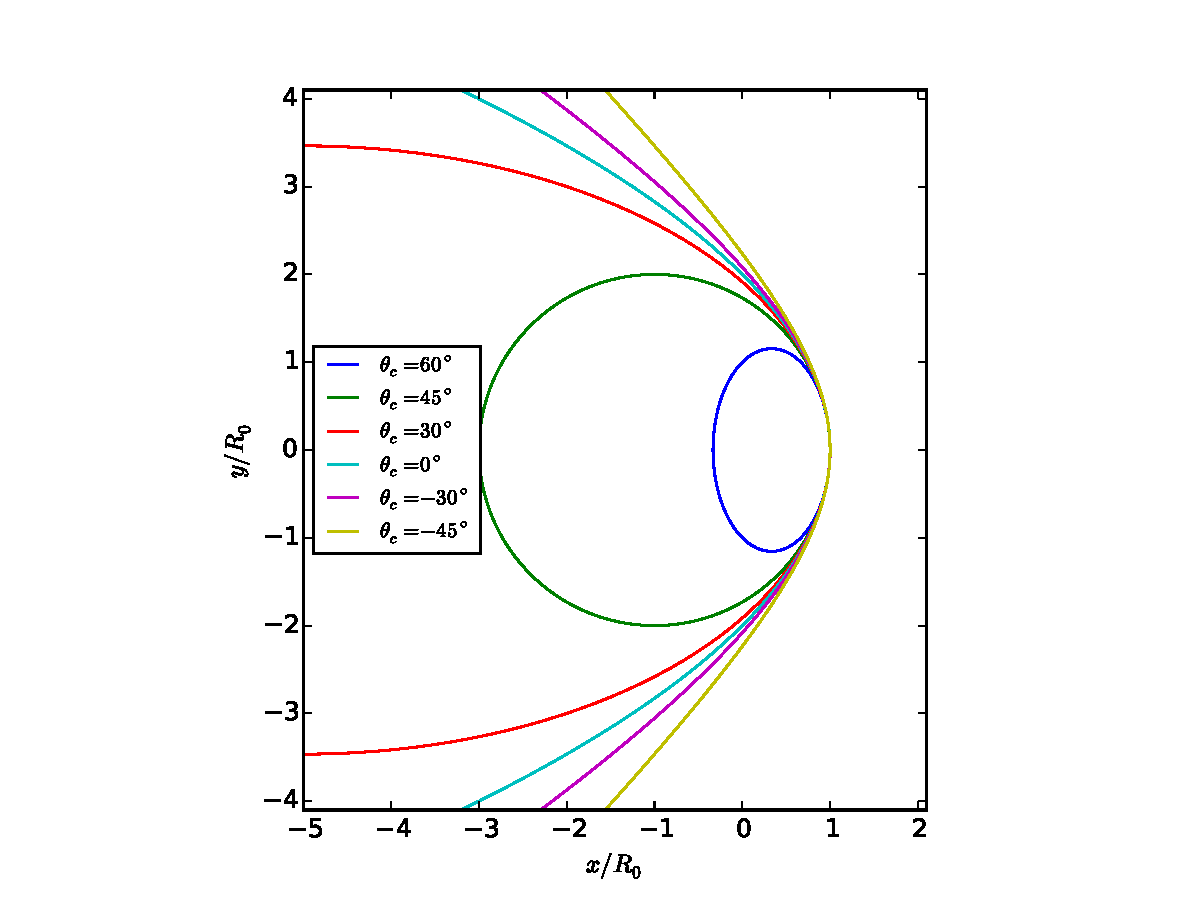
\includegraphics[width=\linewidth]{conic1}
\caption{A whole set of conics with the same radius of curvature. The parameter $\theta_c$ is used as the equivalent of the excentricity. This angle is defined as positive for closed curves
and negative forthe opened ones. An special case is $\theta_c=0$, which describes a parabola.}
\label{fig:conics-family}
\end{figure}
\subsection{Projection onto the plane of sky} 

Once the parametrization is done, we can find the apparent shape of the shell in the observer's frame, following the procedure explained in section \ref{sec:projection}.

First of all, the intrinsic 3D shape of the shell is given by:

\begin{align}
x = a\Cos(t)-x_0 \\ 
y = b\Sin(t)\cos\phi \\
z =  b\Sin(t)\sin\phi
\end{align}

The azimutal angle where the line of sight is tangent to the shell is given by equation (\ref{eq:tanphi}) and (\ref{eq:tanalpha}), then:

\begin{align}
\sin\phi_t &= \frac{b}{a}\tan i\Cot(t) 
\end{align}
where:

\begin{align}
\Cot(t) = \left\lbrace \begin{array}{c}
\cot t ~\mathrm{if~ellipse} \\
-\coth t ~\mathrm{if~hyperbola}
\end{array}\right.
\end{align}

We could work in another frame   where the origin is located at the conic's center: $(X,Y)$, where $X=x-X_0$ and $Y=y$.

In this frame,  we use the transformations (\ref{eq:Trans})  to obtain the apparent shape of the shell:

\begin{align}
X' = \frac{\Cos(t)}{a\cos i}\left(a^2\cos^2 i \pm b^2\sin^2 i\right)  \label{eq:conic-projected-x}\\
Y'= b\Sin(t)\left(1-\frac{b^2}{a^2}\tan^2 i\Cot(t)\right)^{1/2}
\label{eq:conic-projected-y}
\end{align}


We must show that the apparent shape of the shell in the observer's frame is still the same conic. To do that, we can write equations
(\ref{eq:conic-projected-x}) and (\ref{eq:conic-projected-y}) as follows:

\begin{align}
X' = a'\Cos t' \label{eq:conic-projected-x-2} \\
Y' = b'\Sin t' \label{eq:conic-projected-y-2}
\end{align}

Comparing, (\ref{eq:conic-projected-x}), (\ref{eq:conic-projected-x-2}), (\ref{eq:conic-projected-y}) and (\ref{eq:conic-projected-y}) we find that

\begin{align}
a' = \left(a^2\cos^2 i \pm b^2\sin^2 i\right)^{1/2} \\
\Cos(t') = \frac{\Cos(t)}{a\cos i} \\
b' = b
\end{align} 

Which proves that effectively the projection of a given conic is the same conic. With this knowledge, we can obtain the characteristic radii in
the observer's frame.

\begin{align}
D' = D\cos i \\
R'_0 = a' - (a-R_0)\cos i \\
R'_0 = \left(a^2\cos^2 i \pm b^2\sin^2 i\right)^{1/2}  - (a-R_0)\cos i
\end{align}

With  $f(i;\theta_c)\equiv\left(1\pm\tan^2\theta_c\tan^2i\right)^{1/2}$ and introducing the
radius of curvature $R_c\equiv \frac{b^2}{a}$ we find that:

\begin{align}
\frac{R'_0}{D'}=\frac{R_0}{D}\left(1+A\cot^2\theta_c(f(i;\theta_c)-1) \right)
\end{align}

Where $A\equiv \frac{R_c}{R_0}$

The Radius of curvature in the observer's frame is given by $R'_c=\frac{b'^2}{a'}$. Then:

\begin{align}
\frac{R'_c}{R'_0} = \frac{A}{\cos^2 i f(i;\theta_c)\frac{q'}{q}}
\end{align}

Where $q=\frac{R_0}{D}$ and $q' = \frac{R'_0}{D'}$
%Insert figures where needed

%%% Local Variables:
%%% mode: latex
%%% TeX-master: "proplyd-bowshocks"
%%% End:


\newcommand\thC{\(\theta^1\)\,Ori~C}
\defcitealias{Canto:1996}{CRW}
\newcommand\CRW{\citetalias{Canto:1996}}

\section{Application to the hypersonic thin shell solution}
\label{sec:crw-scenario}
As an example application of the ideas of this paper, we consider a
generalization of the thin-shell solution presented in
\citet[][hereafter \CRW{}]{Canto:1996}, for the interaction of two
hypersonic, constant velocity stellar winds.  It is assumed that the
two shocks are highly radiative and that the post-shock flows are
perfectly mixed to form a single shell of negligible thickness.  In
this approximation, the shape of the shell was found algebraically by
\CRW{} from considering conservation of linear and angular momentum,
following an approach first outlined in \citet{Wilkin:1996a}.  The
shape of the bow shock shell is uniquely determined by the parameter
\(\beta\), defined as the momentum-loss ratio of the two winds:
\begin{equation}
  \label{eq:beta-definition}
  \beta \equiv \frac{\dot{M}_w V_w}{\dot{M}_{w1} V_{w1}} . 
\end{equation}
In this definition we use the terminology of \CRW{}, in which
\(\dot{M}_w\) and \(V_w\) are the mass-loss rate and velocity,
respectively, of the wind with source at the origin, while
\(\dot{M}_{w1}\) and \(V_{w1}\) are the mass-loss rate and velocity of
the second wind, located at a distance \(D\) along their \(z\) axis.
Note that \CRW{}'s \(z\) and \(r\) correspond to \(x\) and \(y\) in
sections~\ref{sec:generic-model} to \ref{sec:conic} of the current
paper.  By always placing the weaker of the two winds at the origin,
it is only necessary to consider \(\beta \le 1\).
 
In this work the weakest wind is modeled as an anisotropic hemispherical radial wind
with the following density distribution:

\begin{align}
  n(\theta) = n_0\cos^k\theta
\end{align}  
The index $k$ gives the anisotropy degree. We are interested in winds where $k \geq 0$ for further applications. By the other side, we keep the strongest
wind as isotropic.

The shape of the resultant bow shock is given by:
%If we apply the \CRW{} formalism for a more generalized photoevaporated flow with density given by (\ref{eq:ngen}),
%we find that the solutions for equations (8) - (11) of \CRW{} are the following:

%If we apply the \CRW{} formalism for a generalized photoevaporated flow with density given by equation (\ref{eq:ngen}),
%the shell shape $R(\theta)$ may be calculated from equation (6) of CRW{}:
\begin{align}
  R = \frac{\dot{J}_w + \dot{J}_{w1}}{\left(\dot{\Pi}_{wr}+\dot{\Pi}_{wr1}\right)\cos\theta-\left(\dot{\Pi}_{wz1}+\dot{\Pi}_{wz1}\right)\sin\theta}
  \label{eq:Rmom}
\end{align}

Where:

\begin{align}
\dot{\Pi}_z &= \frac{v_w\dot{M}_w^0}{2(k+2)}\left(1-\cos^{k+2}\theta\right)  \label{eq:pir}\\
\dot{\Pi}_r &= \frac{1}{2}\dot{M}^0_w v_w I_k (\theta) \label{eq:piz}\\
I_k(\theta) & = \int^\theta_0 \cos^k \theta \sin^2\theta~d\theta \label{eq:Ik}\\
\dot{J}_w = 0 \label{eq:jdot} \\
\dot{M}_w &= \frac{\dot{M}_w^0}{2(k+1)}\left(1-\cos^{k+1}\theta\right) \label{eq:dotprop} \\
M^0_w &\equiv 4\pi v_w r^2_{IF} n_0 \bar{m}\\
\dot{\Pi}_{wz1} & = -\frac{\dot{M}^0_{w1}v_{w1}}{4}\sin^2\theta_1\\
\dot{\Pi}_{wr1} & = \frac{\dot{M}^0_{w1}v_{w1}}{4}\left(\theta_1-\sin\theta_1\cos\theta_1\right)\\
\dot{J}_{w1} & = \frac{\dot{M}^0_{w1}v_{w1}}{4}\left(\theta_1-\sin\theta_1\cos\theta_1\right)D \label{eq:jdot1}
\end{align}

Combining equations  (\ref{eq:pir}) to (\ref{eq:jdot1}) we can obtain numerically the bow shock shape $R(\theta)$ from equation (\ref{eq:Rmom}).
To find the projected shape in the plane of sky, we fit $R(\theta)$ into a quadric curve which has the same characteristic radii $(R_0,R_c,R_{90})$. 
%The most notable scenarios, since they have astrophysical relevance are the following:
%$k=1/2$ ak.a. the ``proplyd case'', following \citep{HA:1998}, and $k=0$, ak.a, the ``isotropic case'', following \CRW{}. The comparison between both solutions
%is shown in figure (\ref{fig:r-beta}), along with an extreme anisotropy case. 

\begin{figure}
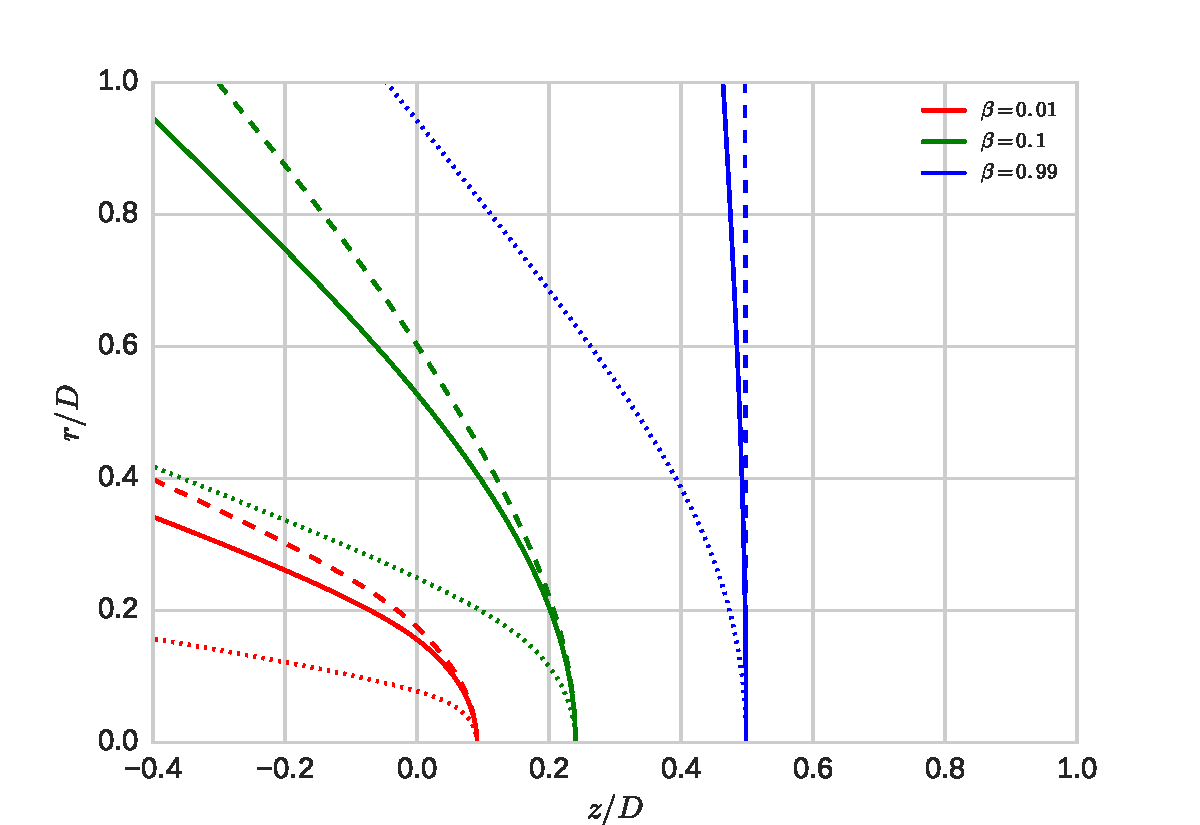
\includegraphics[width=\linewidth]{r-beta}
\caption{Bow shock shapes for interacting winds in the thin-shell
  approximation. Coordinates are normalized by $D$, the distance
  between the two wind sources.  The weaker source is at \((0.0, 0.0)\)
  and the stronger source is at \((1.0, 0.0)\).  Results are shown for
  different values of the wind momentum ratio, \(\beta\), and for the
  case where the weaker wind is isotropic (dashed lines) or an
  anisotropic photoevaporation flow. The solid lines shows a wind with a
  moderate degree of anisotropy $(k=0.5)$, which is expected for the proplyds.
  And the dooted lines show a wind with extreme anisotropy degree $(k=8)$.}
\label{fig:r-beta}
\end{figure}


\subsection{Characteristic Radii}
$R_0$ is obtained directly from equation (27) of \CRW{} as the distance from the inner source where the RAM pressure of the interacting winds is in equilibrium.
%Here goes a little introduction
For the rest of the radii we need a relation between $\theta$ and $\theta_1$ as follows:


\begin{align}
\theta_1\cot\theta_1 -1 = 2\beta I_k(\theta) \cot\theta - \frac{2\beta}{k+2}\left(1-\cos^{k+2}\theta\right)
\label{eq:th1th}
\end{align}

Equation (\ref{eq:th1th}) is reduced to equation (24) of \CRW{} when $k=0$.
We can obtain $R_{90}$ by following the process shown in appendix \ref{app:r90-analytic},
which lead us to a solution for $B \equiv \frac{R_{90}}{R_0}$:

\begin{align}
B = \frac{\sqrt(3\xi)\left(1+\beta^{1/2}\right)}{(1-\xi\beta)\left(1+\frac{1}{5}\xi\beta\right)^{1/2}}
\label{eq:B}
\end{align}

Now, the solution for $R_c$ is explained in appendix \ref{app:rc-analytic},
which lead us to derive the radius of curvature at the symmetry axis:

\begin{align}
R_c &= R_0\left(1-2\gamma\right)^{-1} \label{eq:Rcurv} \\
\mathrm{where:~} & \gamma = \frac{C_{k\beta}}{1+\beta^{1/2}}+\frac{1}{6}(1-2\beta^{1/2})
\end{align}

Finally, using equations (\ref{eq:Rcurv}) and (\ref{eq:B}) we can estimate the parameter of
conic curves $\theta_c$ as a function of $(\beta,\xi)$ using equation (\ref{eq:thc-conic})

\begin{align}
\tan^2\theta_c &= \left| \frac{3\xi\left(1+\beta^{1/2}\right)^2}{\left(1-\xi\beta\right)^2\left(1+\frac{1}{5}\xi\beta\right)}-\frac{2}{\left(1-2\gamma\right)}\right| 
\label{eq:thc-CRW}
\end{align}

\begin{figure}
\begin{tabular}{c}
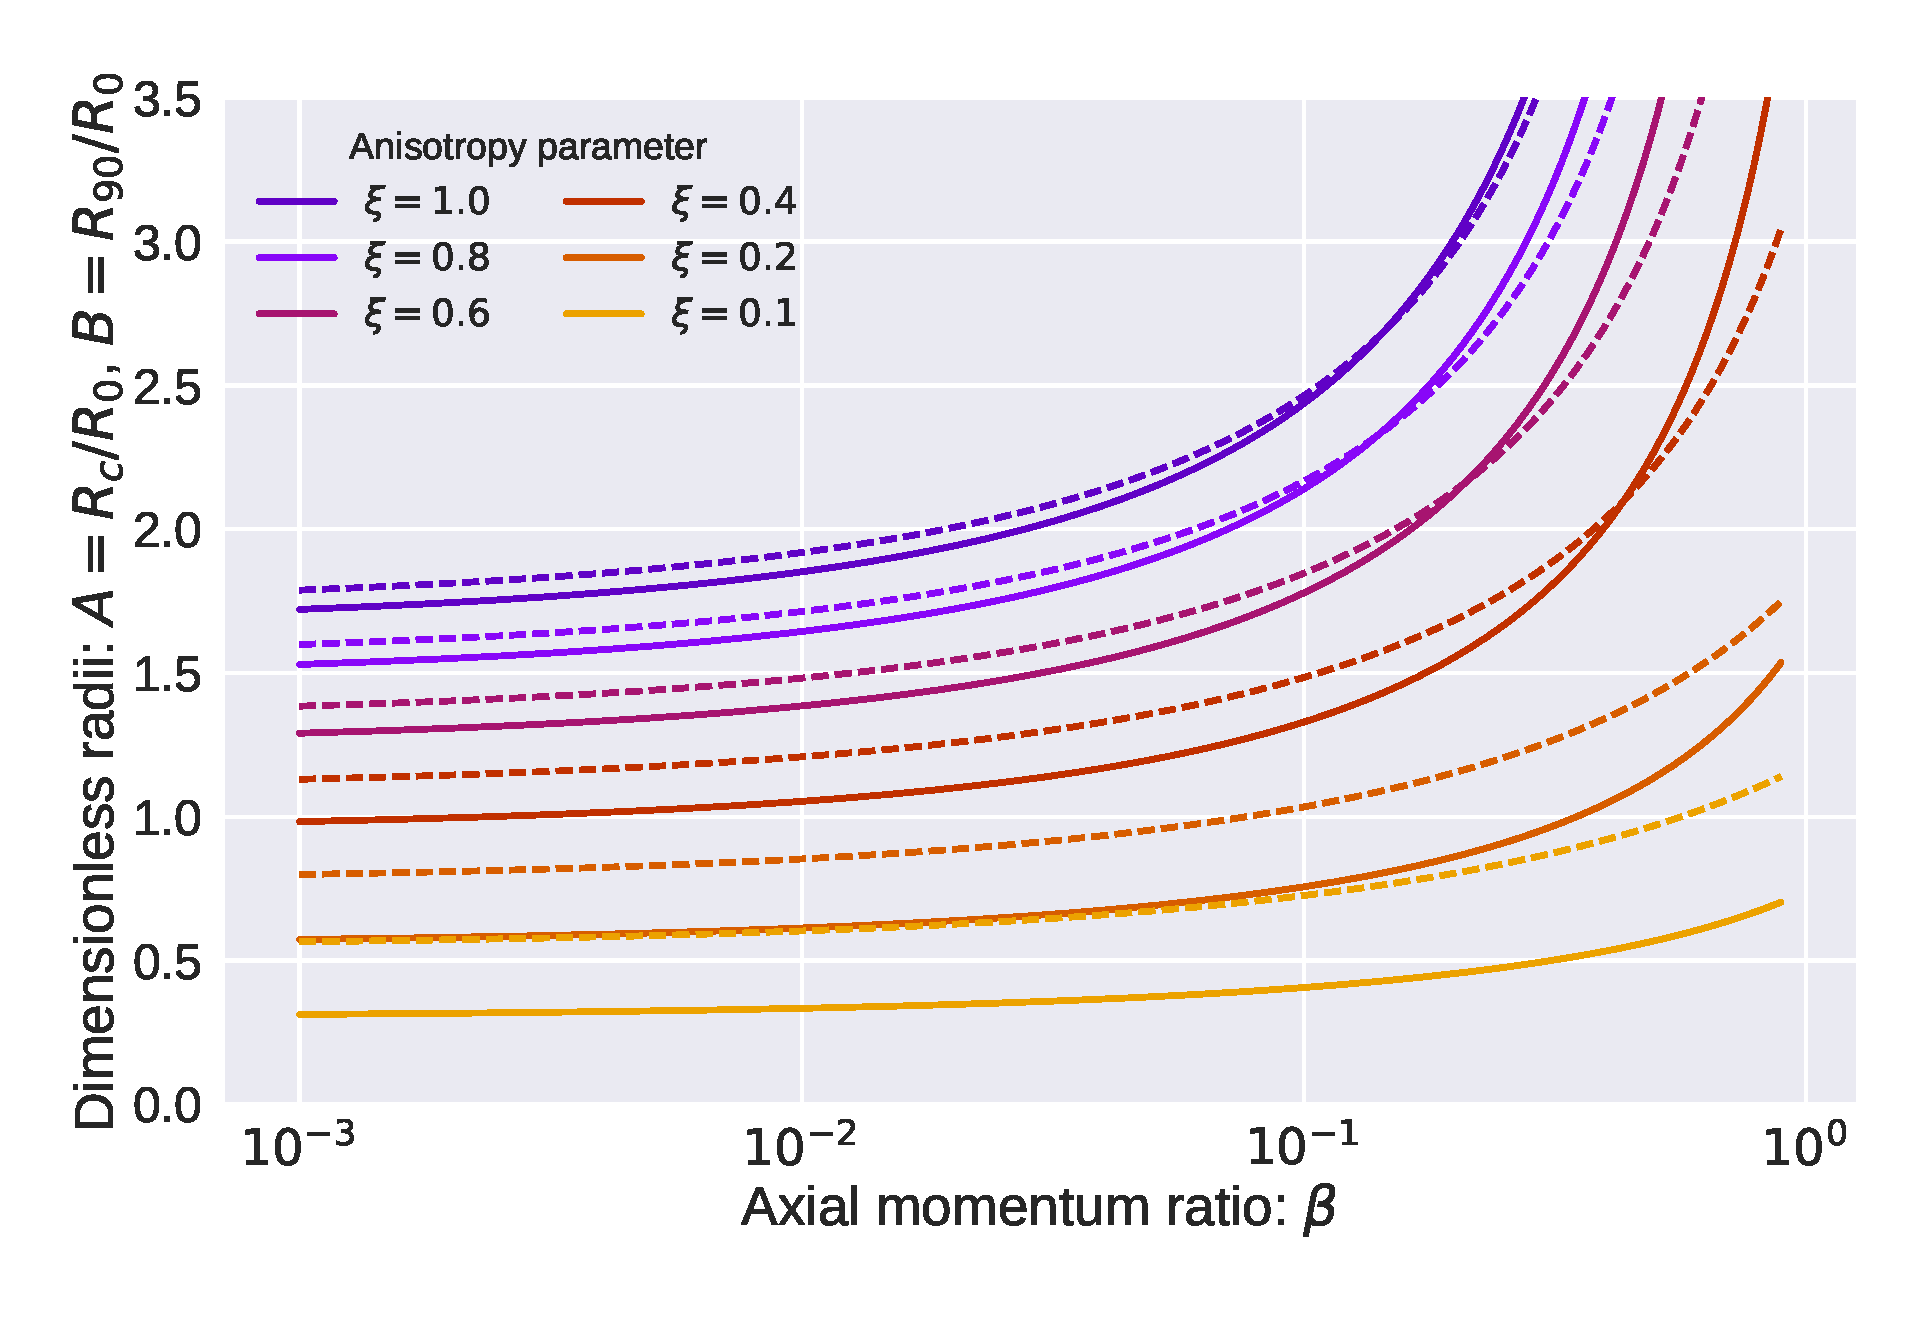
\includegraphics[width=\linewidth]{figs/AB-beta-log} \\
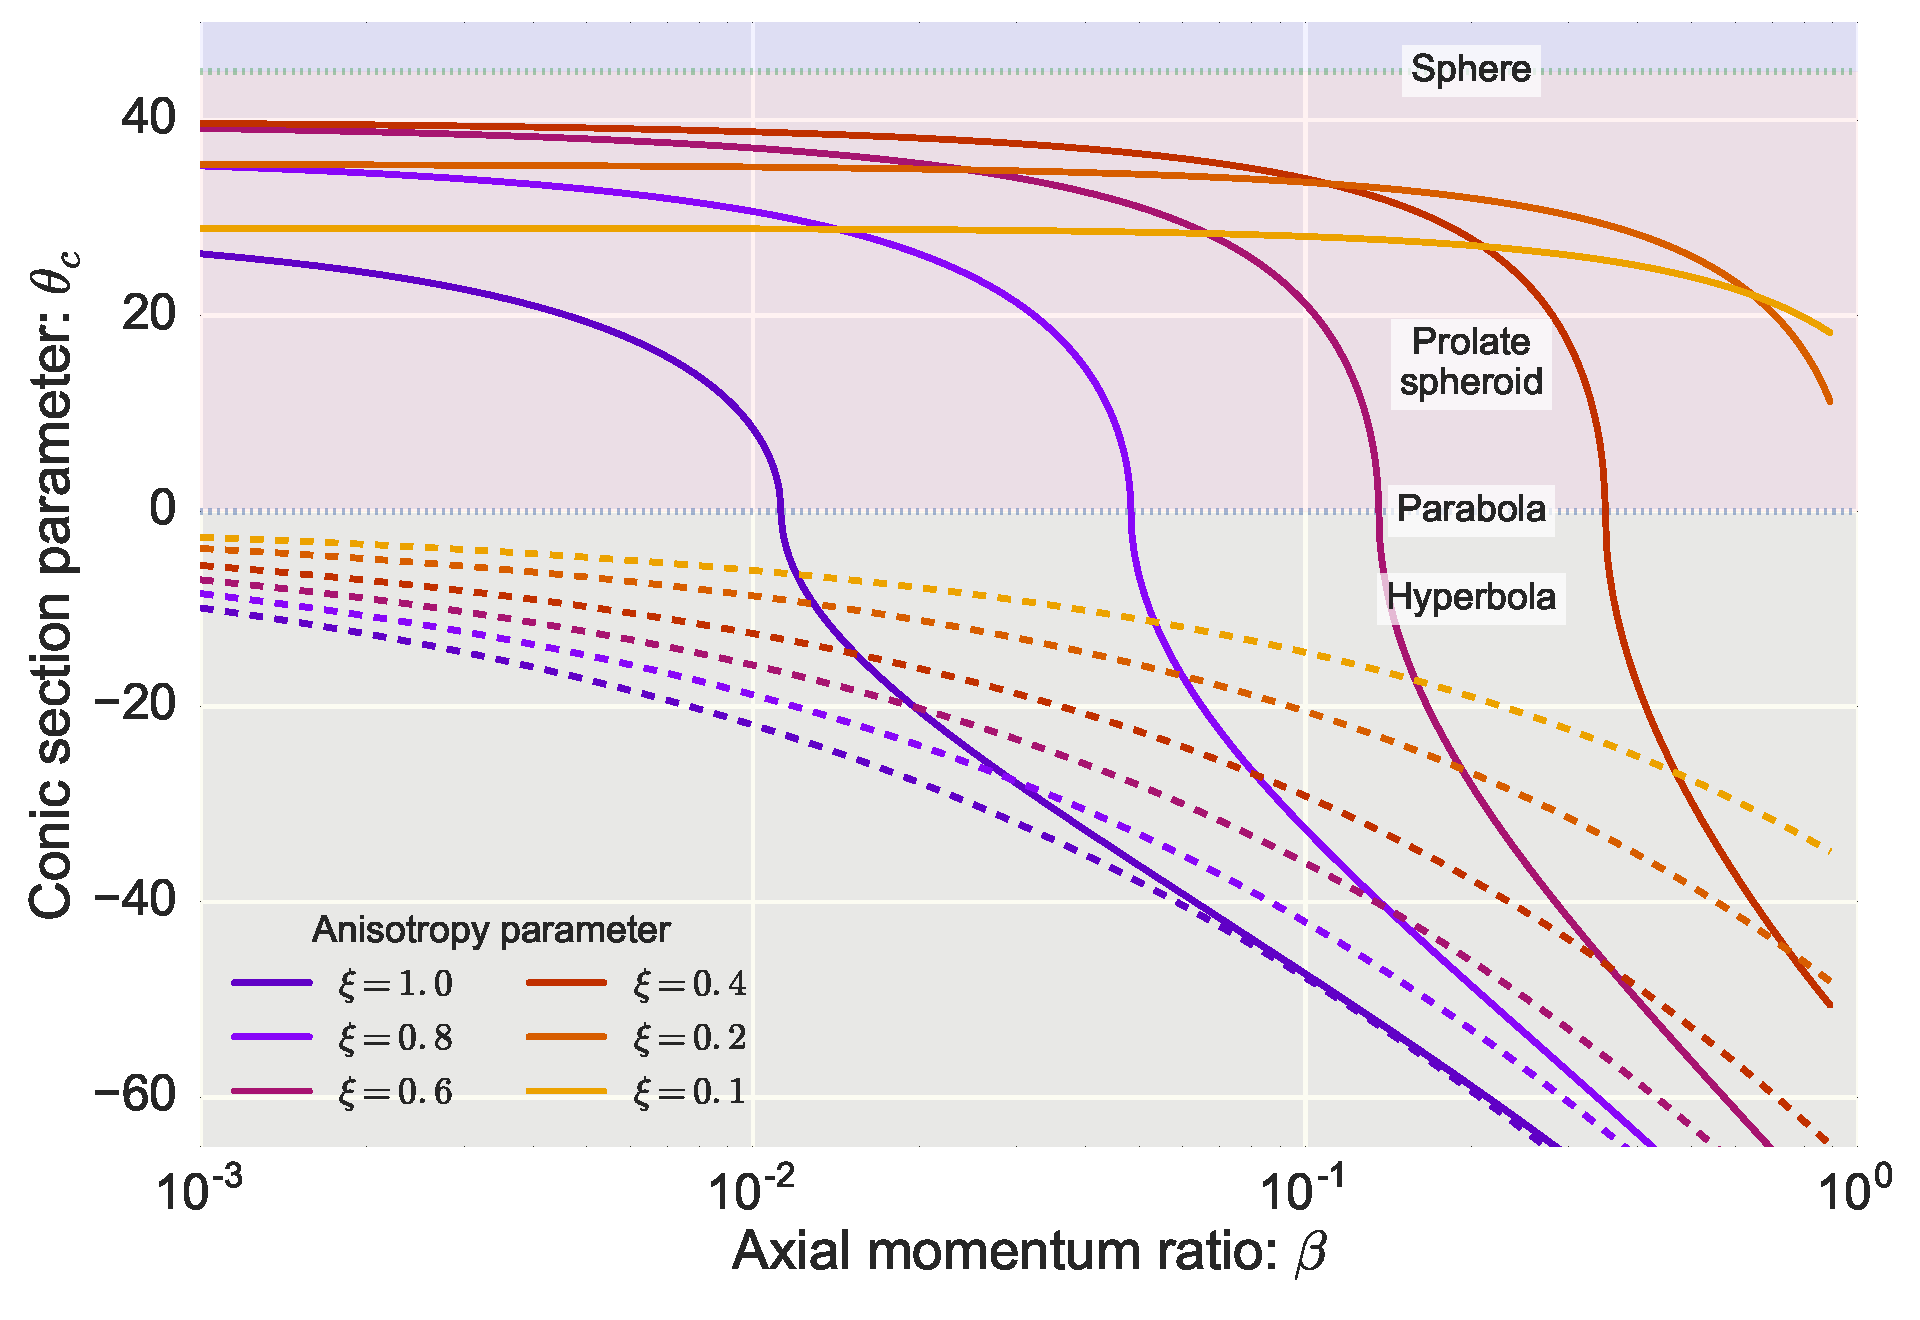
\includegraphics[width=\linewidth]{figs/thc-beta-log}
\end{tabular}
\caption{Top: Characteristic radii, $A = R_c/R_0$ (solid lines) and $B
  = R_{90}/R_0$ (dashed lines)
  vs $\beta$, calculated from quadric fits to the generalized CRW
  solutions with varying degrees of isotropy $\xi$.  Bottom: Conic
  angle $\theta_c$ vs $\beta$ for the bow 
  shock head (solid lines) and the bow shock tail (dashed lines).}
\label{fig:rad-beta}
\end{figure}


%Observationally, we can measure the projected radii. In order to estimate the model parameters is neccesary to measure at least two of the mentioned radii, being $R_0$ the
%easiest to measure. Therefore, we may compare both $R_c$ and $R_{90}$ against $R_0$ as shown in figure (\ref{fig:prop-shell-rad}). 

With this we can use the results of section \ref{sec:conic} to estimate the projected conic shapes for bow shocks with different winds 
momenta and different density distributions. Figure \ref{fig:rad-beta} shows equations ( \ref{eq:B}), (\ref{eq:Rcurv}) and (\ref{eq:thc-CRW}) for different anisotropy indexes. 


\subsection{Fits to the tail}
\label{sec:fits-tail}


For the hyperbola ``center''
\begin{multline}
  \label{eq:tail-analytic-x0}
  x_{0,\mathrm{t}} = 0.7 \beta^{-0.55} \biggl[
    C_3 \bigl(\log_{10}\beta\bigr)^3 + C_2 \bigl(\log_{10}\beta\bigr)^2 
  \\ + C_1 \log_{10}\beta + C_0
  \biggr]
\end{multline}
\begin{equation}
  \label{eq:tail-analytic-x0-minus-a}
  (x_{0,\mathrm{t}} - a_{\mathrm{t}}) = D_2 (\log_{10}\beta)^2 + D_1 \log_{10}\beta + D_0
\end{equation}
where
\begin{alignat}{2}
  C_k &= c_{2,k} \xi^2 + c_{1,k} \xi + c_{0,k} &\quad \text{for\ } k &= \{0, 1, 2, 3\} \\
  D_k &= d_{2,k} \xi^2 + d_{1,k} \xi + d_{0,k} &\quad \text{for\ } k &= \{0, 1, 2\} \\
  \label{eq:tail-analytic-coeffs}
\end{alignat}


\newcommand\iso{\ensuremath{^{\mathrm{iso}}}}

\begin{table}
  \caption{Coefficients for hyperbola fit to bowshock tails}
  \label{tab:tail-fit-coeffs}
  \begin{align*}
  C\iso_0 & = {0.123}  & c_{0,0} & = {0.123} & c_{1,0} & = {0.123} & c_{2,0} & = {0.123} \\
  C\iso_1 & = {0.123}  & c_{0,1} & = {0.123} & c_{1,1} & = {0.123} & c_{2,1} & = {0.123} \\
  C\iso_2 & = {0.123}  & c_{0,2} & = {0.123} & c_{1,2} & = {0.123} & c_{2,2} & = {0.123} \\
  C\iso_3 & = {0.123}  & c_{0,3} & = {0.123} & c_{1,3} & = {0.123} & c_{2,3} & = {0.123} \\
  D\iso_0 & = {0.123}  & d_{0,0} & = {0.123} & d_{1,0} & = {0.123} & d_{2,0} & = {0.123} \\
  D\iso_1 & = {0.123}  & d_{0,1} & = {0.123} & d_{1,1} & = {0.123} & d_{2,1} & = {0.123} \\
  D\iso_2 & = {0.123}  & d_{0,2} & = {0.123} & d_{1,2} & = {0.123} & d_{2,2} & = {0.123} \\
  \end{align*}
\end{table}




\begin{figure*}
  \centering
  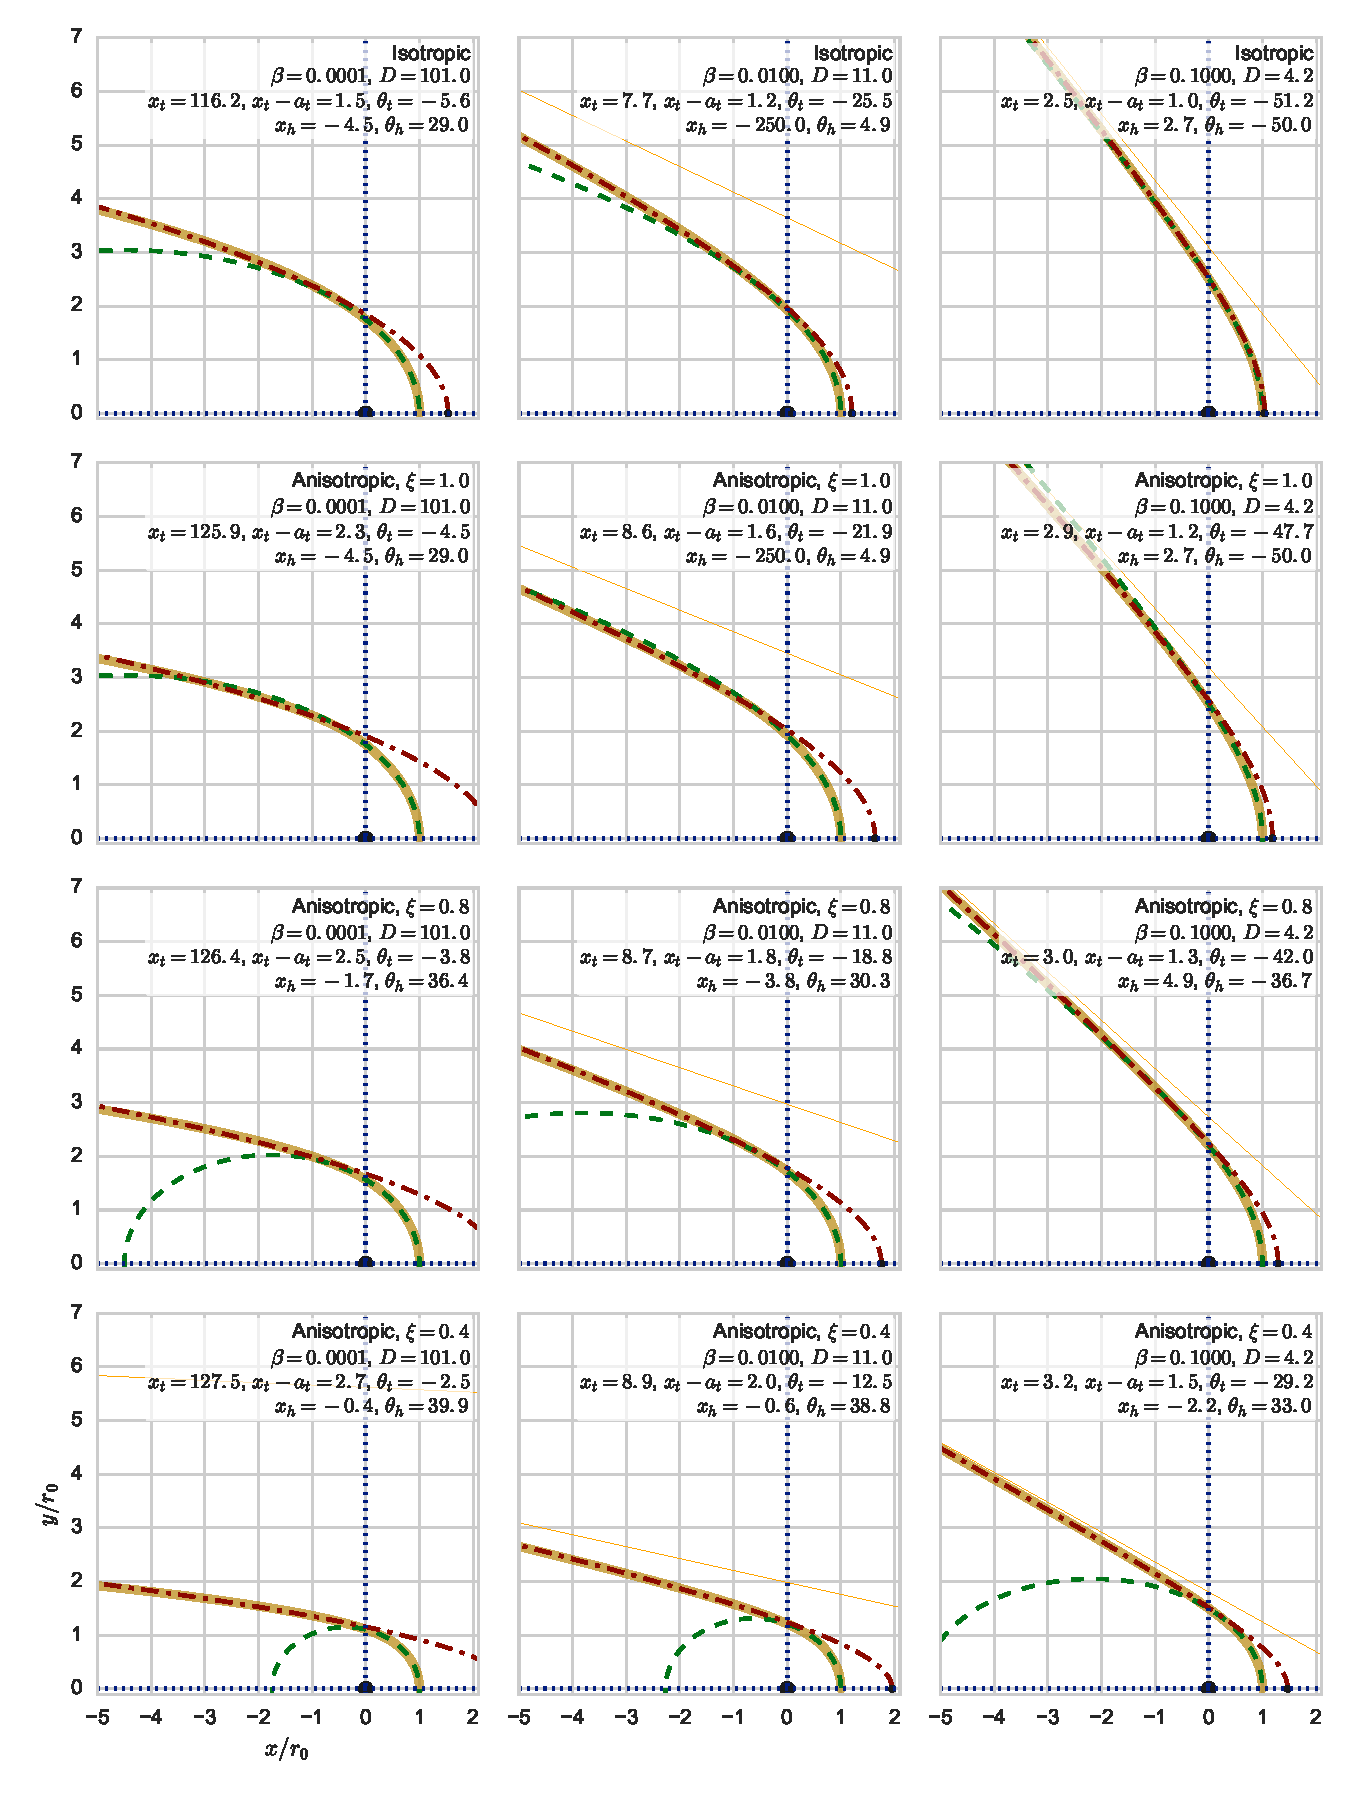
\includegraphics[width=\linewidth]{figs/conic-head-tail-fit}
  \caption{Double quadric fits to thin shell
    solutions. \textit{Replace these with a version that uses analytic
    fit to tail hyperbola parameters}}
  \label{fig:head-tail}
\end{figure*}

%%% Local Variables:
%%% mode: latex
%%% TeX-master: "quadrics-bowshock"
%%% End:

\section{Conclusions}
\label{sec:conc}

%\newcommand\thC{\(\theta^1\)\,Ori~C}
\defcitealias{Canto:1996}{CRW}

We developed a method to estimate the shape of a generic bow shock product of the
interaction of two winds and was applied to the proplyds in the core of the ONC.
We started measuring the projected characteristic radii $(R'_0,R'_c)$ for each proplyd in our
sample and compare them with the ``conic equivalent'' of a two winds interaction model based 
on \CRW{} work to estimate the intrinsic bow shock shape and get the ionizing flux for ionization balance 
and the stagnation pressure for our sample of proplyds.
Most results are consistent with a proplyd's photoevaporated flow with an anisotropic density
distribution, with different anisotropy degrees. We ound that LV4 has the least anisotropic flow,
while LV2 has the most anisotropic flow. And for the 177-341, 169-348 and 180-331 we found out that 
the stellar wind is not enough to keep their bow socks stationary.

%%% Local Variables:
%%% mode: latex
%%% TeX-master: "proplyd-bowshocks"
%%% End:

\bibliographystyle{mnras}
%% All references should be put in the BibTeX file bowshocks-biblio.bib
\bibliography{bowshocks-biblio}
\appendix
% \appendixpage
% \addappheadtotoc
\section{Parabola of Revolution}
\label{app:parabola}

In this section we develop the particular case of the parabola.
The parametrization is given by:

\begin{align}
x &= - \frac{1}{2}R_ct^2 + R_0 \\
y &= R_c t
\end{align}
Where $R_c$ is the radius of curvature and $R_0$ is the distance of the parabola nose to the
origin.
The respective tridimensional shape is given by:
\begin{align}
x &= -\frac{1}{2}R_ct^2 + R_0 \label{eq:x-par-a}\\
y &= R_c t \cos\phi  \label{eq:y-par-a}\\
z &= R_c t \sin\phi  \label{eq:z-par-a}
\end{align}
The azimutal angle where the surface is tangent to the line of sight in this case is given by:
\begin{align}
\sin\phi_t = -\frac{\tan i}{t} \label{eq:sin-tan-a} 
\end{align}

Subtituting (\ref{eq:sin-tan-a}) into (\ref{eq:x-par-a}), (\ref{eq:y-par-a}) and
(\ref{eq:z-par-a}) we find the apparent shape
of the paraboloid:

\begin{align}
x' &= -\frac{R_c(\frac{1}{2}t^2 \cos^2 i -\sin^2 i)}{\cos i}+R_0\cos i \\
y' &= R_c\left(t^2-\tan^2 i\right)^{1/2} 
\end{align}

Taking the limit of equations (\ref{eq:qprime}) and (\ref{eq:Aprime}) when $\theta_c$ tends to zero we find that:

\begin{align}
\left(\frac{q'}{q}\right)_{\mathrm{parabola}} &= 1+\frac{\tilde{R}_c\tan^2 i}{2}\\
\left(\tilde{R}'_c\right)_{\mathrm{parabola}} &= \frac{\tilde{R}_c}{\cos^2 i + \frac{\tilde{R}_c}{2}\sin^2 i}
\end{align}

\section{Analytic derivation of the radius of curvature in the Thin Shell model}
\label{app:rc-analytic}

For small $\theta$ we may do a polynomial expansion for the shell shape such as:

\begin{align}
R \simeq R_0\left(1+\gamma\theta^2 + \Gamma\theta^4\right) \label{eq:R-exp}
\end{align}

The radius of curvature at the axis for $R$ is given by:

\begin{align}
R_c = R_0\left(1-2\gamma\right)^{-1}
\end{align}

The coefficient gamma may be derived by an expansion at small angles of equation
(\ref{eq:th1th}), as follows:

From the first term of the right side we get:

\begin{align}
\cot\theta &\simeq \theta^{-1}\left[1-\frac{1}{3}\theta^2\right] \\
\cos^k\theta\sin^2\theta &\simeq \theta^2 - \left(\frac{1}{3} + \frac{k}{2}\right)\theta^4 \\
\implies I_k(\theta) &\simeq \frac{1}{3}\theta^3\left[ 1 - \frac{1}{10}(3k+2)\theta^2\right]\\
\implies 2\beta I_k(\theta)\cot\theta &\simeq \frac{2}{3}\beta\theta^2\left[1-\frac{1}{30}
(9k+16)\theta^2\right]\label{eq:AR1} 
\end{align}

For the second term we get:

\begin{align}
-\frac{2\beta}{k+2}\left(1-\cos^{k+2}\theta\right) & \simeq -\beta\theta^2\left[1-\frac{1}{12}
(3k+4)\theta^2\right] \label{eq:AR2}
\end{align}

For the left side we use equation (25) from \CRW{}. Then, equation (\ref{eq:th1th}) results
as follows:

\begin{align}
\theta_1^2\left(1+\frac{1}{15}\theta_1^2\right) = \beta\theta^2\left[1+\frac{1}{60}(4-9k)
\theta^2\right] \label{eq:th1th-app}
\end{align}

And we can use the approximation $\theta_1 \approx \beta\theta^2$ for the correction term in
the left side of (\ref{eq:th1th-app}):

\begin{align}
\theta_1^2 &= \beta\theta^2\left[1+\frac{1}{60}(4-9k)\theta^2\right]
\left(1-\frac{\beta}{15}\theta^2\right) \\
\implies \theta_1^2 &= \beta\theta^2\left[1+ 2C_{k\beta}\theta^2\right]
\label{eq:th1th-small}\\
\mathrm{where:~} C_{k\beta} &\equiv \frac{1}{2}\left(A_k-\frac{\beta}{15}\right) \\
A_k &\equiv \frac{1}{15}-\frac{3k}{20}
\end{align}

Now, using equation (23) from \CRW{} we may estimate $R$ at low angles. To do this, we need to
expand each term as follows (neglecting terms of order four or higher):

\begin{align}
\theta_1 = &= \beta^{1/2}\theta\left[1+ 2C_{k\beta}\theta^2\right]^{1/2} \\
\theta + \theta_1 &= \theta\left[1+\beta^{1/2}\left(1+2C_{k\beta}\theta^2\right)\right]\\
\sin\theta_1 &= \theta_1\left[1-\frac{\theta_1^2}{6}\right] \\
 &= \beta^{1/2}\theta\left[1+\left(C_{k\beta}-\frac{1}{6}\beta\right)\theta^2\right] \\
 \sin(\theta+\theta_1) &= \left[\theta+\theta_1\right]\left[1-\frac{\left(\theta+\theta_1
 \right)^2}{6}\right] \\
 &= \theta\left(1+\beta^{1/2}\right)\left\lbrace 1+\left[\frac{C_{k\beta}\beta^{1/2}}
 {1+\beta^{1/2}}-\frac{1}{6}\left(1+\beta^{1/2}\right)^2\right]\theta^2\right\rbrace
\end{align}


So, combining these terms with equation (23) from \CRW{} we found the final expression for $R$:

\begin{align}
\frac{R}{D}\equiv \frac{\sin\theta_1}{\sin(\theta+\theta_1)} = \frac{\beta^1/2}{1+\beta^{1/2}}
\left\lbrace 1 + \theta^2\left[\frac{C_{k\beta}}{1+\beta^{1/2}}+\frac{1}{6}\left(1+2\beta^{1/2}
\right)\right] \right\rbrace \label{eq:r-small-theta}
\end{align}

Returning to equation (\ref{eq:R-exp}) we see the following:

\begin{align}
R_0 &= \frac{\beta^{1/2}}{1+\beta^{1/2}} \\
\gamma &= \frac{C_{k\beta}}{1+\beta^{1/2}}+\frac{1}{6}\left(1+2\beta^{1/2}\right)
\label{eq:app-gamma}
\end{align}

We recover equation (27) of \CRW{} for $R_0$ and equation (\ref{eq:app-gamma}) is the
needed term to calculate the radius of curvature at the axis.

\section{Analytic derivation of \texorpdfstring{\boldmath $R_{90}$}{R\_90} in the thin shell model}
\label{app:r90-analytic}

To derive $R_{90}$ we need to evaluate equations (23) from \CRW{} and (\ref{eq:th1th})
at $\theta=\frac{\pi}{2}$:

\begin{align}
R_{90} = D\tan\theta_{1,90} \\
\theta_{1,90}\cot\theta_{1,90} -1 = -\frac{2\beta}{k+2} \label{eq:th190}
\end{align}
Where $\theta_{1,90}\equiv \theta_1(\frac{\pi}{2})$. Combining both equations and  introducing
the parameter $\xi\equiv \frac{2}{k+2}$ we have:
\begin{align}
R_{90} &= D\frac{\theta_{1,90}}{1-\xi\beta} \label{eq:r90-incomplete}
\end{align}

Expanding the left side of (\ref{eq:th190}) until fourth order, equation (\ref{eq:th190})
becomes:

\begin{align}
\theta_{1,90}^2\left(1+\frac{\theta_{1,90}^2}{15}\right) \simeq 3\xi\beta
\end{align}

Applying the approximation $\theta_1^2 \approx 3\xi\beta$ we found a solution
for $\theta_{1,90}$:

\begin{align}
\theta_{1,90} = \left(\frac{3\xi\beta}{1+\frac{1}{5}\xi\beta}\right)^{1/2}
\end{align}

And substituting into (\ref{eq:r90-incomplete}) we find the solution for $R_{90}$:

\begin{align}
R_{90} &= \frac{\left(3\xi\beta\right)^{1/2}}{\left(1+\frac{1}{5}\xi\beta\right)^{1/2}
\left(1-\xi\beta\right)} \\
\implies \tilde{R}_{90} &\equiv \frac{R_{90}}{R_0} = \frac{\sqrt{3\xi}\left(1+\beta^{1/2}\right)}
{\left(1+\frac{1}{5}\xi\beta\right)^{1/2}\left(1-\xi\beta\right)}
\end{align}

\section{Derivation of Characteristic Radii in Isotropic Wind/Parallel interaction Problem}
\label{app:ch-rad-Wilkin}

$\tilde{R}_{90}$ is obtained by simply evaluating equation (\ref{eq:R-Wilkin}) at $\theta=\frac{\pi}{2}$.
For the Radius of curvature we follow a similar procedure than the Wind/Wind interaction, but using equation
(\ref{eq:R-Wilkin}) for $R(\theta)$ and inserting the cosecant into the square root.

Expanding the terms of $R(\theta)$ we find the following:

\begin{align}
  \csc^2\theta &\simeq \theta^{-2}\left[1+\frac{\theta^2}{3}\left(1+\frac{\theta^2}{5}\right)\right] \\
  1-\theta\cot\theta &\simeq \frac{\theta^2}{3}\left[1 + \frac{\theta^2}{15}\left(1+\frac{2\theta^2}{21}\right)\right] \\
  \implies \tilde{R}(\theta) \simeq 1 + \frac{\theta^2}{5} + O\left[\theta^4\right]
\end{align}

From equation (\ref{eq:Rcurv}) for the radius of curvature we finally get the numerical value for $\tilde{R_c} = \frac{5}{3}$
\clearpage

% Landscape table needs to go on its own page, so we need to manually
% adjust the section counter so that it will ``belong'' to the next
% section
\addtocounter{section}{1}
\sisetup{detect-all=true, detect-inline-weight=math}
\sisetup{round-mode=figures, round-precision=2}
\begin{landscape}
\begin{table}
  \setlength\tabcolsep{3pt}
  \caption{Results of all statistical tests performed on observed bow shock shape parameters. Significant correlations are shown in \textbf{bold}, marginally significant correlations in \textit{italic}}
  \label{tab:big-p}
  %%% MIPSGAL summary statistics
%%% Table automatically generated from mipsgal-summary-stats.tab
%%% 2017-06-08 14:17:39.847703
%%%
% \Width is used to align number under col header in first column
	\newlength\Width\settowidth\Width{Comparison}
	\begin{tabular}{@{} ll @{\quad } S[round-mode=places]S[round-mode=places] S[round-mode=places]S[round-mode=places] SS SS @{\quad\quad\quad} SSS[round-mode=places] @{\quad} S@{}S@{}S @{}}\toprule
	  & {Dependent} & \multicolumn{2}{c}{Mean} & \multicolumn{2}{c}{Std.\ Dev.} & \multicolumn{2}{c}{Obs.\ Disp.} & \multicolumn{2}{c @{\quad\quad\quad}}{s.e.m.} & \multicolumn{3}{c @{\quad} }{\dotfill Effect sizes\dotfill } & \multicolumn{3}{c}{\dotfill Non-parametric test \(p\)-values  \dotfill} \\ 
	  {Comparison} & {Variable} & {\(\langle \text{A} \rangle\)} & {\(\langle \text{B} \rangle\)} & {\(\sigma_{\text{A}}\)} & {\(\sigma_{\text{B}}\)} & {\(\langle \epsilon_{\text{A}} \rangle\)} & {\(\langle \epsilon_{\text{B}} \rangle\)} & {\((\sigma/\!\sqrt n)_{\text{A}}\)} & {\((\sigma/\!\sqrt n)_{\text{B}}\)} & {\(r_b\)} & {Cohen \(d\)} & {\(\sigma_{\text{A}}/\sigma_{\text{B}}\)} & \multicolumn{1}{c}{Anderson--Darling} & \multicolumn{1}{c}{Rank biserial} &  \multicolumn{1}{c}{Brown--Forsythe}\\
	  {\makebox[\Width]{(1)}} & \multicolumn{1}{c@{\quad}}{(2)} & {(3)} & {(4)} & {(5)} & {(6)} & {(7)} & {(8)} & {(9)} & {(10)}  & {(11)} & {(12)} & {(13)} & {(14)} & {(15)} & {(16)} \\  
	  \midrule\multicolumn{10}{@{} l @{\quad\quad\quad}}{\itshape Median split of continuous independent variables \dotfill}\\
\addlinespace
Faint/bright & \(R_{90} / R_{0}\) & 1.677 & 1.768 & 0.269 & 0.316 & 0.231 & 0.236 & 0.025 & 0.03 & \itshape 0.174 & \itshape 0.308 & 1.175 & \itshape 0.0215 & \itshape 0.0235 & 0.125\\
\(H\) magnitude & \(\Delta R_{90} / R_{90}\) & 0.183 & 0.198 & 0.161 & 0.163 &   &   & 0.015 & 0.015 & 0.07 & 0.093 & 1.013 & 0.538 & 0.365 & 0.761\\
\(n_{\text{A}} =  n_{\text{B}} = 113\) & \(R_{c} / R_{0}\) & 1.655 & 1.917 & 0.631 & 1.045 & 0.097 & 0.078 & 0.059 & 0.098 & 0.123 & 0.303 & \itshape 1.654 & 0.123 & 0.111 & \itshape 0.0335\\
\addlinespace
Low/high & \(R_{90} / R_{0}\) & 1.707 & 1.739 & 0.25 & 0.336 & 0.256 & 0.212 & 0.024 & 0.031 & 0.061 & 0.11 & \bfseries 1.342 & \itshape 0.0281 & 0.428 & \bfseries 0.00139\\
bow shock size, \(R_0\) & \(\Delta R_{90} / R_{90}\) & 0.175 & 0.204 & 0.157 & 0.165 &   &   & 0.015 & 0.015 & 0.091 & 0.176 & 1.054 & 0.103 & 0.238 & 0.193\\
\(n_{\text{A}} =  n_{\text{B}} = 113\) & \(R_{c} / R_{0}\) & 1.766 & 1.803 & 0.975 & 0.755 & 0.114 & 0.062 & 0.092 & 0.071 & 0.1 & 0.043 & 0.774 & 0.228 & 0.192 & 0.599\\
\addlinespace
Low/high & \(R_{90} / R_{0}\) & 1.703 & 1.742 & 0.267 & 0.323 & 0.233 & 0.235 & 0.025 & 0.03 & 0.04 & 0.132 & 1.213 & 0.554 & 0.602 & 0.123\\
extinction, \(A_K\) & \(\Delta R_{90} / R_{90}\) & 0.186 & 0.195 & 0.138 & 0.183 &   &   & 0.013 & 0.017 & -0.039 & 0.057 & 1.326 & 0.301 & 0.61 & 0.112\\
\(n_{\text{A}} =  n_{\text{B}} = 113\) & \(R_{c} / R_{0}\) & 1.725 & 1.846 & 0.822 & 0.917 & 0.091 & 0.085 & 0.077 & 0.086 & 0.082 & 0.139 & 1.116 & 0.219 & 0.285 & 0.982\\
\addlinespace
Low/high & \(R_{90} / R_{0}\) & 1.722 & 1.724 & 0.328 & 0.261 & 0.234 & 0.234 & 0.031 & 0.024 & 0.02 & 0.008 & 0.796 & 0.308 & 0.795 & 0.0534\\
\(\vert{}b\vert\) & \(\Delta R_{90} / R_{90}\) & 0.188 & 0.191 & 0.161 & 0.162 &   &   & 0.015 & 0.015 & 0.009 & 0.021 & 1.005 & 0.964 & 0.907 & 0.694\\
\(n_{\text{A}} =  n_{\text{B}} = 113\) & \(R_{c} / R_{0}\) & 1.706 & 1.862 & 0.727 & 0.988 & 0.085 & 0.091 & 0.068 & 0.092 & 0.069 & 0.181 & 1.358 & 0.19 & 0.368 & 0.0842\\
\addlinespace
High/low & \(R_{90} / R_{0}\) & 1.734 & 1.707 & 0.279 & 0.321 & 0.241 & 0.223 & 0.024 & 0.034 & -0.049 & -0.093 & 1.152 & 0.361 & 0.532 & 0.159\\
\(\cos \ell\) & \(\Delta R_{90} / R_{90}\) & 0.182 & 0.201 & 0.155 & 0.171 &   &   & 0.013 & 0.018 & 0.054 & 0.122 & 1.1 & 0.604 & 0.491 & 0.365\\
\(n_{\text{A}}, n_{\text{B}} = 137, 90\) & \(R_{c} / R_{0}\) & 1.807 & 1.751 & 0.946 & 0.742 & 0.09 & 0.084 & 0.081 & 0.078 & -0.0 & -0.064 & 0.785 & 1.03 & 0.999 & 0.549\\
\midrule
\multicolumn{10}{@{} l @{\quad\quad\quad}}{\itshape Categorical independent variables \dotfill}\\
\addlinespace
Environment: & \(R_{90} / R_{0}\) & 1.735 & 1.693 & 0.283 & 0.338 & 0.238 & 0.218 & 0.022 & 0.053 & -0.07 & -0.142 & 1.194 & 0.603 & 0.49 & 0.392\\
Isolated vs Facing & \(\Delta R_{90} / R_{90}\) & 0.19 & 0.195 & 0.161 & 0.172 &   &   & 0.012 & 0.027 & -0.019 & 0.034 & 1.066 & 0.507 & 0.85 & 0.438\\
\(n_{\text{A}}, n_{\text{B}} = 170, 41\) & \(R_{c} / R_{0}\) & 1.757 & 1.852 & 0.854 & 0.899 & 0.087 & 0.083 & 0.066 & 0.14 & 0.042 & 0.11 & 1.053 & 0.713 & 0.676 & 0.377\\
\addlinespace
Environment: & \(R_{90} / R_{0}\) & 1.735 & 1.68 & 0.283 & 0.309 & 0.238 & 0.233 & 0.022 & 0.077 & -0.13 & -0.193 & 1.092 & 0.518 & 0.391 & 0.782\\
Isolated vs \hii & \(\Delta R_{90} / R_{90}\) & 0.19 & 0.175 & 0.161 & 0.138 &   &   & 0.012 & 0.034 & -0.048 & -0.095 & 0.855 & 0.932 & 0.754 & 0.799\\
\(n_{\text{A}}, n_{\text{B}} = 170, 16\) & \(R_{c} / R_{0}\) & 1.757 & 1.907 & 0.854 & 0.955 & 0.087 & 0.105 & 0.066 & 0.239 & 0.024 & 0.174 & 1.118 & 0.496 & 0.875 & 0.255\\
\addlinespace
Single/multiple & \(R_{90} / R_{0}\) & 1.709 & 1.762 & 0.289 & 0.315 & 0.23 & 0.243 & 0.022 & 0.041 & 0.074 & 0.177 & 1.09 & 0.342 & 0.396 & 0.338\\
source candidate & \(\Delta R_{90} / R_{90}\) & 0.184 & 0.206 & 0.162 & 0.16 &   &   & 0.013 & 0.021 & 0.093 & 0.136 & 0.987 & 0.421 & 0.284 & 0.97\\
\(n_{\text{A}}, n_{\text{B}} = 167, 60\) & \(R_{c} / R_{0}\) & 1.767 & 1.833 & 0.825 & 0.988 & 0.09 & 0.08 & 0.064 & 0.128 & 0.027 & 0.076 & 1.198 & 0.999 & 0.756 & 0.605\\
\addlinespace
With/without & \(R_{90} / R_{0}\) & 1.734 & 1.721 & 0.289 & 0.298 & 0.223 & 0.237 & 0.043 & 0.022 & -0.042 & -0.044 & 1.031 & 0.595 & 0.667 & 0.563\\
\SI{8}{\um} emission & \(\Delta R_{90} / R_{90}\) & 0.203 & 0.186 & 0.205 & 0.149 &   &   & 0.031 & 0.011 & 0.021 & -0.106 & 0.726 & 0.765 & 0.826 & 0.219\\
\(n_{\text{A}}, n_{\text{B}} = 45, 182\) & \(R_{c} / R_{0}\) & 1.714 & 1.802 & 0.598 & 0.926 & 0.091 & 0.087 & 0.089 & 0.069 & -0.012 & 0.101 & 1.547 & 0.824 & 0.904 & 0.2\\
\addlinespace
3-star vs (4+5)-star & \(R_{90} / R_{0}\) & 1.661 & 1.812 & 0.288 & 0.286 & 0.247 & 0.216 & 0.025 & 0.029 & \bfseries 0.328 & \bfseries 0.525 & 0.99 & \bfseries 8.23e-05 & \bfseries 2.63e-05 & 0.403\\
 & \(\Delta R_{90} / R_{90}\) & 0.189 & 0.19 & 0.162 & 0.161 &   &   & 0.014 & 0.017 & -0.007 & 0.009 & 0.994 & 0.809 & 0.927 & 0.561\\
\(n_{\text{A}}, n_{\text{B}} = 133, 94\) & \(R_{c} / R_{0}\) & 1.632 & 2.0 & 0.91 & 0.764 & 0.106 & 0.061 & 0.079 & 0.079 & \bfseries 0.386 & \bfseries 0.431 & 0.84 & \bfseries 1.47e-05 & \bfseries 7.66e-07 & 0.762\\
\midrule
\multicolumn{10}{@{} l @{\quad\quad\quad}}{\itshape Intercomparison with other datasets \dotfill}\\
\addlinespace
MIPS vs Orion & \(R_{90} / R_{0}\) & 1.723 & 2.418 & 0.297 & 0.811 &   &   & 0.02 & 0.191 & \bfseries 0.7 & \bfseries 1.928 & \bfseries 2.735 & \bfseries 8.02e-06 & \bfseries 7.84e-07 & \bfseries 6.41e-06\\
 & \(\Delta R_{90} / R_{90}\) & 0.19 & 0.701 & 0.162 & 0.532 &   &   & 0.011 & 0.148 & \bfseries 0.689 & \bfseries 2.553 & \bfseries 3.29 & \bfseries 9.94e-06 & \bfseries 3e-05 & \bfseries 2.42e-10\\
\(n_{\text{A}}, n_{\text{B}} = 227, 18\) & \(R_{c} / R_{0}\) & 1.784 & 2.639 & 0.871 & 1.302 &   &   & 0.058 & 0.307 & \bfseries 0.516 & \bfseries 0.94 & 1.495 & \bfseries 0.000505 & \bfseries 0.000273 & 0.12\\
\addlinespace
MIPS vs RSG & \(R_{90} / R_{0}\) & 1.723 & 1.402 & 0.297 & 0.092 &   &   & 0.02 & 0.035 & \bfseries -0.742 & \bfseries -1.098 & \itshape 0.311 & \bfseries 0.000571 & \bfseries 0.000841 & \itshape 0.0406\\
 & \(\Delta R_{90} / R_{90}\) & 0.19 & 0.15 & 0.162 & 0.087 &   &   & 0.011 & 0.033 & -0.072 & -0.247 & 0.539 & 0.795 & 0.747 & 0.286\\
\(n_{\text{A}}, n_{\text{B}} = 227, 7\) & \(R_{c} / R_{0}\) & 1.784 & 1.437 & 0.871 & 0.083 &   &   & 0.058 & 0.031 & -0.191 & -0.405 & 0.095 & 0.0798 & 0.392 & 0.053
\\
\bottomrule
\end{tabular}

\end{table}
\end{landscape}
\begin{table}
  \contcaption{Results of all statistical tests performed on observed
    bow shock shape parameters.}
  \begin{tabular}{p{0.9\linewidth}}
    \toprule
    \textit{Description of columns:}
    (Col.~1)~How the two A/B source sub-samples are defined, also giving the size of each sub-sample, \(n_{\text{A}}\) and~\(n_{\text{B}}\).
    (Col.~2)~Dependent variable whose distribution is compared between the two sub-samples.
    (Cols.~3--6)~Mean and standard deviation, \(\sigma\), of the dependent variable for each of the two sub-samples.
    (Cols.~7--8)~Mean over each sub-sample of the observational dispersion (\(\epsilon\), standard deviation) of radii that contribute to the dependent variable for each individual source.
    (Cols.~9--10)~``Standard error of the mean'' (s.e.m.) of the dependent variable for each of the two sub-samples. 
    (Cols.~11--13)~Standardized ``effect sizes'', which are dimensionless measures of the difference in the distribution of the dependent variable between the two sub-samples.
    (Col.~11)~Rank biserial correlation coefficient \citep{Cureton:1956a}, which is obtained by considering all \(n_{\text{A}} n_{\text{B}}\) pair-wise comparisons of the dependent variable between a source in sub-sample~A and a source in sub-sample~B.  It is the difference between the fraction of such comparisons ``won'' by sub-sample~A and those ``won'' by sub-sample~B, and thus may vary between \(-1\) and \(+1\). 
    (Col.~12)~Cohen's \(d\), which is a dimensionless mean difference: \(d = (\langle \text{A} \rangle - \langle \text{B} \rangle) / \sigma_{\text{pool}} \), where \(\sigma_{\text{pool}} = (n_{\text{A}} \sigma_{\text{A}}^2 + n_{\text{B}} \sigma_{\text{B}}^2)^{1/2} / \sqrt{n_{\text{A}} + n_{\text{B}}}\) is the pooled standard deviation.
    (Col.~13)~Ratio of standard deviations between the two sub-samples.
    (Cols.~14--16)~Probabilities (\(p\)-values) of the two sub-samples being as different as observed if they were to be drawn from the same population, according to three different non-parametric tests.
    (Col.~14)~Anderson--Darling 2-sample test, which is a general test of similarity between two distributions that is designed to retain sensitivity to differences in the tails of the distributions.
    (Col.~15)~Mann--Whitney--Wilcoxon \(U\) test \citep{Mann:1947a}, which is sensitive 
    (Col.~16)~Brown--Forsythe test for equality of variance \citep{Brown:1974a}
    \\
    \bottomrule
  \end{tabular}
\end{table}

\addtocounter{section}{-1}

\section{Distribution of p-values for all correlations tested}
\label{sec:distr-p-values}
\addtocounter{table}{1}


\begin{figure}
  (a)\\
  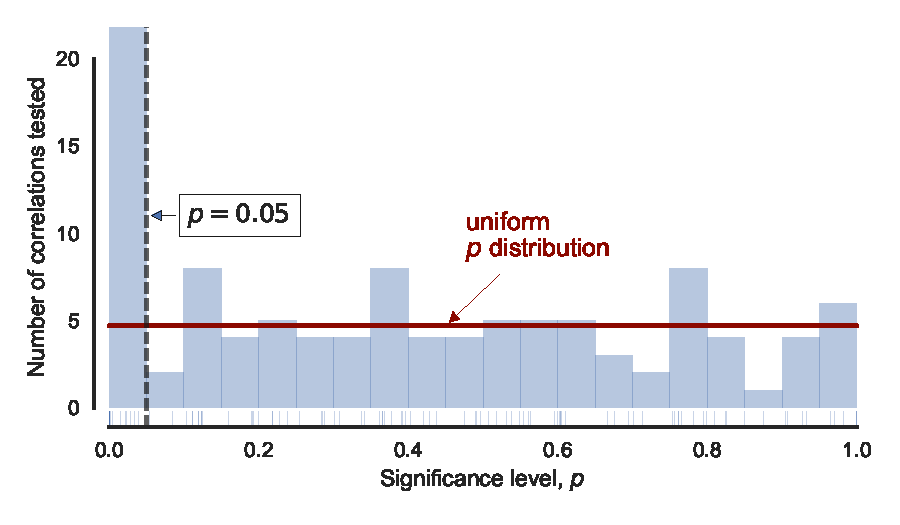
\includegraphics[width=\linewidth]{figs/p-value-histogram-new-linear}\\
  (b)\\
  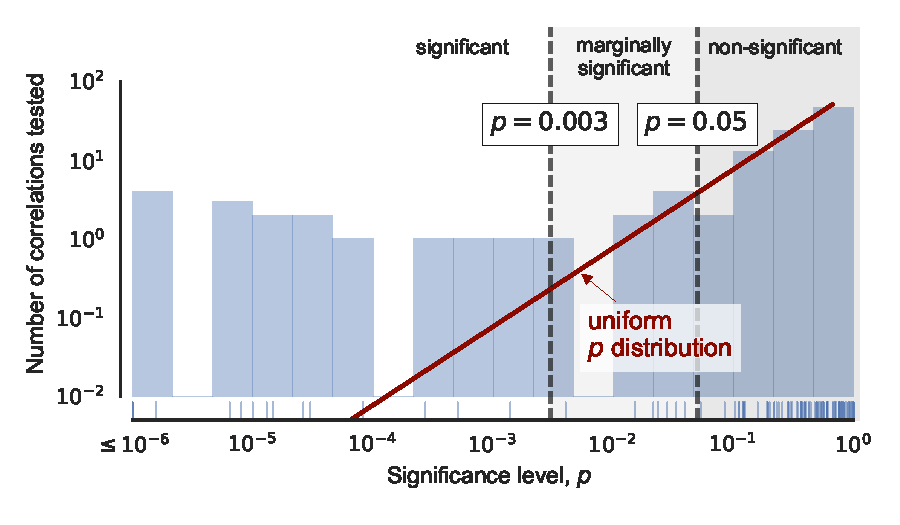
\includegraphics[width=\linewidth]{figs/p-value-histogram-new}
  \caption{Histogram of \(p\)-values for all non-parametric 2-sample
    tests listed in Table~\ref{tab:big-p}. (a)~Uniformly spaced linear
    bins and linear vertical axis. (b)~Uniformly spaced logarithmic
    bins and logarithmic vertical axis, with all values
    \(p \le 10^{-6}\) included in the leftmost bin.  The vertical dashed
    lines shows the traditional threshold values for significance:
    \(p = 0.001\) and \(p = 0.05\). The red solid line shows the
    uniform distribution of \(p\)-values that would be expected if the
    null hypothesis were always true, that is, if no significant
    correlations existed.}
  \label{fig:histo-p-values}
\end{figure}


Results from all the statistical tests discussed in \S~\ref{sec:corr-shape} are given in Table~\ref{tab:big-p}.  


\begin{table}
  \caption{Lower bounds on the Type~I error rate, \(\alpha\)}
  \label{tab:type-I}
  \centering
  \begin{tabular}{lrr} \toprule
    Correlation & \(p\) & \(\alpha\) \\
    \midrule
    \multicolumn{3}{l}{\itshape Quantitative \dotfill}\\
    \(R_c\) vs \(R_0\) & \textit{0.0054} & \textit{0.0712} \\
    \(R_{90}\) vs \(R_0\) & \textbf{0.0001} & \textbf{0.0025} \\
    \(R_c\) vs \(H_0\) & 0.1229 & 0.4119 \\
    \(R_{90}\) vs \(H_0\) & \textit{0.0215} & \textit{0.1833} \\
    \(R_c\) vs \(A_K\) & 0.19 & 0.4617 \\
    \(R_{90}\) vs \(A_K\) & 0.63 & 1 \\
    \(R_c\) vs \(|b|\) & 0.19 & 0.4617 \\
    \(R_{90}\) vs \(|b|\) & 0.31 & 0.4967 \\
    \(R_c\) vs \(\cos(\ell)\) & 1.00 & 1 \\
    \(R_{90}\) vs \(\cos(\ell)\) & 0.36 & 0.4999 \\
    \midrule
    \multicolumn{3}{l}{\itshape Categorical} \dotfill\\
    \(R_c\) vs Facing & 0.71 & 1 \\
    \(R_c\) vs H II & 0.50 & 1 \\
    \(R_{90}\) vs Facing & 0.60 & 1 \\
    \(R_{90}\) vs H II & 0.52 & 1 \\
    \(R_c\) vs Multiple & 1.00 & 1 \\
    \(R_{90}\) vs Multiple & 0.34 & 0.4993 \\
    \(R_c\) vs \SI{8}{\um} & 0.82 & 1 \\
    \(R_{90}\) vs \SI{8}{\um} & 0.6 & 1 \\
    \midrule
    \multicolumn{3}{l}{\itshape Other datasets} \dotfill\\
    \(R_c\) vs Herschel & 0.074 & 0.3437 \\
    \(R_{90}\) vs Herschel & \textbf{0.00052} & \textbf{0.0106} \\
    \(R_c\) vs M42 & \textbf{0.00048} & \textbf{0.0099} \\
    \(R_{90}\) vs M42 & \textbf{0.0000105} & \textbf{0.0003} \\
    \bottomrule
  \end{tabular}
\end{table}


The \(p\)-values are the probability of finding a difference between
two populations as large as (or larger than) what is observed,
\emph{given} that there is no difference in the underlying
distribution from which the two populations are drawn (that is, given
that the null hypothesis is true).  However, what we really want to
know is something else: the probability that the null hypothesis is
true, \emph{given} the observations.  That is, the probability,
\(\alpha\), of a \textit{false positive}, also known as the \textit{Type I
  error rate}.  The common mistake of conflating these two definitions
is known as the ``\(p\)-value fallacy'' \citep{Goodman:1999a}, or``the
error of the transposed conditional'', as discussed in detail by
\citet{Colquhoun:2014a}.  It is possible to derive \(\alpha\) from
\(p\) using Bayes' theorem (e.g., \citealp{Goodman:1999b}), but that
requires an estimate of the prior probability of the null hypothesis,
independent of the observations.  Alternatively, it is also possible
to find a lower bound on \(\alpha\) from a frequentist approach
\citep{Sellke:2001a}:
\begin{equation}
  \label{eq:type-I}
  \alpha(p) \ge \bigg[ 1 - \big(e\, p \ln p\big)^{-1} \bigg]^{-1}
  \quad \text{valid for } p < 1/e.
\end{equation}
This is the approach we adopt here, which also numerically coincides
with the Bayesian approach for the case where the prior probability of
the null hypothesis is 0.5.  The reason that this is only a lower
limit for \(\alpha\) is that if we have overwhelming a priori evidence that
the null hypothesis is true (for instance, from previous empirical
studies, or because it follows from a well-supported theory), then a
Bayesian calculation would give a much higher value of \(\alpha\) than
\eqref{eq:type-I} does.  In our case, however, we have no strong
reasons for favoring any of the null hypotheses, so it is reasonable
to assume \(\alpha\) is close to the lower limit given in \eqref{eq:type-I}.

In order to choose a threshold \(p\)-value that counts as a
``significant'' result, one then needs to balance the risks of false
positives against the risks of \textit{false negatives}.  The false
negative probability, \(\beta\), also known as \textit{Type II error
  rate}, is the probability of failing to reject an untrue null
hypothesis.  That is, in the context of this paper, it is the
probability of failing to detect a real difference between two
sub-samples, or a real correlation between two variables.  The
complementary probability, \(1 - \beta\), is known as the
\textit{statistical power} or sensitivity of the test.  The value of
\(\beta\) depends on three factors:
\begin{enumerate}[1.]
\item The \textit{effect size}, which is a measure of the magnitude of
  the difference in a dependent variable between two sub-samples, or
  the degree of correlation between two continuous variables.  For the
  two sub-sample case, it is common to use a standardised mean
  difference, such as Cohen's \(d\) statistic \citep{Cohen:1988a}:
  \(d = (\bar{X}_A - \bar{X}_B) / s\), where \(\bar{X}_A\),
  \(\bar{X}_B\) are the means of the dependent variable \(X\) for
  samples A and B, while \(s\) is the pooled standard deviation of
  \(X\).  For the case of two continuous variables, the Pearson linear
  correlation coefficient, \(r\), can be used.  In both cases, rules
  of thumb have been developed \citep{Ruscio:2008a} for classifying an
  effect as ``large'' (\(d > 0.8\), \(r > 0.4\)) or ``small''
  (\(d < 0.2\), \(r < 0.1\)).  Alternatively, non-parametric
  statistics can be used, such as the \(A\) measure of stochastic
  superiority \citep{Delaney:2002a}.
\end{enumerate}

Obviously, this depends on the \textit{effect size}, which is the 


All astronomical data analysis is \emph{post hoc} analysis, since the universe was not set up to test a particular hypothesis (as far as we know).  It is therefore important to guard against the ``multiple comparisons problem'', whereby seemingly significant correlations are found where none really exist, simply by virtue of the large number of tests that were carried out.

Under the more conservative Holm--Bonferroni method, only comparisons with \(p < 0.001\) would be significant. 

The p-curve \citep{Head:2015a}

%%% Local Variables:
%%% mode: latex
%%% TeX-master: "quadrics-bowshock.tex"
%%% End:


\end{document}

%%% Local Variables:
%%% mode: latex
%%% TeX-master: t
%%% End:

